% Options for packages loaded elsewhere
\PassOptionsToPackage{unicode}{hyperref}
\PassOptionsToPackage{hyphens}{url}
%
\documentclass[
]{book}
\usepackage{amsmath,amssymb}
\usepackage{lmodern}
\usepackage{iftex}
\ifPDFTeX
  \usepackage[T1]{fontenc}
  \usepackage[utf8]{inputenc}
  \usepackage{textcomp} % provide euro and other symbols
\else % if luatex or xetex
  \usepackage{unicode-math}
  \defaultfontfeatures{Scale=MatchLowercase}
  \defaultfontfeatures[\rmfamily]{Ligatures=TeX,Scale=1}
\fi
% Use upquote if available, for straight quotes in verbatim environments
\IfFileExists{upquote.sty}{\usepackage{upquote}}{}
\IfFileExists{microtype.sty}{% use microtype if available
  \usepackage[]{microtype}
  \UseMicrotypeSet[protrusion]{basicmath} % disable protrusion for tt fonts
}{}
\makeatletter
\@ifundefined{KOMAClassName}{% if non-KOMA class
  \IfFileExists{parskip.sty}{%
    \usepackage{parskip}
  }{% else
    \setlength{\parindent}{0pt}
    \setlength{\parskip}{6pt plus 2pt minus 1pt}}
}{% if KOMA class
  \KOMAoptions{parskip=half}}
\makeatother
\usepackage{xcolor}
\IfFileExists{xurl.sty}{\usepackage{xurl}}{} % add URL line breaks if available
\IfFileExists{bookmark.sty}{\usepackage{bookmark}}{\usepackage{hyperref}}
\hypersetup{
  pdftitle={Análises Ecológicas no R: Exercícios e Soluções},
  hidelinks,
  pdfcreator={LaTeX via pandoc}}
\urlstyle{same} % disable monospaced font for URLs
\usepackage{color}
\usepackage{fancyvrb}
\newcommand{\VerbBar}{|}
\newcommand{\VERB}{\Verb[commandchars=\\\{\}]}
\DefineVerbatimEnvironment{Highlighting}{Verbatim}{commandchars=\\\{\}}
% Add ',fontsize=\small' for more characters per line
\usepackage{framed}
\definecolor{shadecolor}{RGB}{248,248,248}
\newenvironment{Shaded}{\begin{snugshade}}{\end{snugshade}}
\newcommand{\AlertTok}[1]{\textcolor[rgb]{0.94,0.16,0.16}{#1}}
\newcommand{\AnnotationTok}[1]{\textcolor[rgb]{0.56,0.35,0.01}{\textbf{\textit{#1}}}}
\newcommand{\AttributeTok}[1]{\textcolor[rgb]{0.77,0.63,0.00}{#1}}
\newcommand{\BaseNTok}[1]{\textcolor[rgb]{0.00,0.00,0.81}{#1}}
\newcommand{\BuiltInTok}[1]{#1}
\newcommand{\CharTok}[1]{\textcolor[rgb]{0.31,0.60,0.02}{#1}}
\newcommand{\CommentTok}[1]{\textcolor[rgb]{0.56,0.35,0.01}{\textit{#1}}}
\newcommand{\CommentVarTok}[1]{\textcolor[rgb]{0.56,0.35,0.01}{\textbf{\textit{#1}}}}
\newcommand{\ConstantTok}[1]{\textcolor[rgb]{0.00,0.00,0.00}{#1}}
\newcommand{\ControlFlowTok}[1]{\textcolor[rgb]{0.13,0.29,0.53}{\textbf{#1}}}
\newcommand{\DataTypeTok}[1]{\textcolor[rgb]{0.13,0.29,0.53}{#1}}
\newcommand{\DecValTok}[1]{\textcolor[rgb]{0.00,0.00,0.81}{#1}}
\newcommand{\DocumentationTok}[1]{\textcolor[rgb]{0.56,0.35,0.01}{\textbf{\textit{#1}}}}
\newcommand{\ErrorTok}[1]{\textcolor[rgb]{0.64,0.00,0.00}{\textbf{#1}}}
\newcommand{\ExtensionTok}[1]{#1}
\newcommand{\FloatTok}[1]{\textcolor[rgb]{0.00,0.00,0.81}{#1}}
\newcommand{\FunctionTok}[1]{\textcolor[rgb]{0.00,0.00,0.00}{#1}}
\newcommand{\ImportTok}[1]{#1}
\newcommand{\InformationTok}[1]{\textcolor[rgb]{0.56,0.35,0.01}{\textbf{\textit{#1}}}}
\newcommand{\KeywordTok}[1]{\textcolor[rgb]{0.13,0.29,0.53}{\textbf{#1}}}
\newcommand{\NormalTok}[1]{#1}
\newcommand{\OperatorTok}[1]{\textcolor[rgb]{0.81,0.36,0.00}{\textbf{#1}}}
\newcommand{\OtherTok}[1]{\textcolor[rgb]{0.56,0.35,0.01}{#1}}
\newcommand{\PreprocessorTok}[1]{\textcolor[rgb]{0.56,0.35,0.01}{\textit{#1}}}
\newcommand{\RegionMarkerTok}[1]{#1}
\newcommand{\SpecialCharTok}[1]{\textcolor[rgb]{0.00,0.00,0.00}{#1}}
\newcommand{\SpecialStringTok}[1]{\textcolor[rgb]{0.31,0.60,0.02}{#1}}
\newcommand{\StringTok}[1]{\textcolor[rgb]{0.31,0.60,0.02}{#1}}
\newcommand{\VariableTok}[1]{\textcolor[rgb]{0.00,0.00,0.00}{#1}}
\newcommand{\VerbatimStringTok}[1]{\textcolor[rgb]{0.31,0.60,0.02}{#1}}
\newcommand{\WarningTok}[1]{\textcolor[rgb]{0.56,0.35,0.01}{\textbf{\textit{#1}}}}
\usepackage{longtable,booktabs,array}
\usepackage{calc} % for calculating minipage widths
% Correct order of tables after \paragraph or \subparagraph
\usepackage{etoolbox}
\makeatletter
\patchcmd\longtable{\par}{\if@noskipsec\mbox{}\fi\par}{}{}
\makeatother
% Allow footnotes in longtable head/foot
\IfFileExists{footnotehyper.sty}{\usepackage{footnotehyper}}{\usepackage{footnote}}
\makesavenoteenv{longtable}
\usepackage{graphicx}
\makeatletter
\def\maxwidth{\ifdim\Gin@nat@width>\linewidth\linewidth\else\Gin@nat@width\fi}
\def\maxheight{\ifdim\Gin@nat@height>\textheight\textheight\else\Gin@nat@height\fi}
\makeatother
% Scale images if necessary, so that they will not overflow the page
% margins by default, and it is still possible to overwrite the defaults
% using explicit options in \includegraphics[width, height, ...]{}
\setkeys{Gin}{width=\maxwidth,height=\maxheight,keepaspectratio}
% Set default figure placement to htbp
\makeatletter
\def\fps@figure{htbp}
\makeatother
\setlength{\emergencystretch}{3em} % prevent overfull lines
\providecommand{\tightlist}{%
  \setlength{\itemsep}{0pt}\setlength{\parskip}{0pt}}
\setcounter{secnumdepth}{5}
\usepackage{booktabs}
\ifLuaTeX
  \usepackage{selnolig}  % disable illegal ligatures
\fi
\usepackage[]{natbib}
\bibliographystyle{apalike}

\title{Análises Ecológicas no R: Exercícios e Soluções}
\author{}
\date{\vspace{-2.5em}2022-02-11}

\begin{document}
\maketitle

{
\setcounter{tocdepth}{1}
\tableofcontents
}
\hypertarget{sobre}{%
\chapter*{Sobre}\label{sobre}}

Aqui você encontra os \textbf{exercícios e soluções} do livo \href{https://analises-ecologicas.netlify.app/}{Análises Ecológicas no R}.

\hypertarget{cap.-4---introduuxe7uxe3o-ao-r}{%
\chapter*{Cap. 4 - Introdução ao R}\label{cap.-4---introduuxe7uxe3o-ao-r}}
\addcontentsline{toc}{chapter}{Cap. 4 - Introdução ao R}

\textbf{4.1}
Use o R para verificar o resultado da operação \texttt{7\ +\ 7\ ÷\ 7\ +\ 7\ x\ 7\ -\ 7}.

Solução:

\begin{Shaded}
\begin{Highlighting}[]
\DecValTok{7} \SpecialCharTok{+} \DecValTok{7} \SpecialCharTok{/} \DecValTok{7} \SpecialCharTok{+} \DecValTok{7} \SpecialCharTok{*} \DecValTok{7} \SpecialCharTok{{-}} \DecValTok{7}
\CommentTok{\#\textgreater{} [1] 50}
\end{Highlighting}
\end{Shaded}

\textbf{4.2}
Verifique através do R se \texttt{3x2³} é maior que \texttt{2x3²}.

Solução:

\begin{Shaded}
\begin{Highlighting}[]
\DecValTok{3} \SpecialCharTok{*} \DecValTok{2}\SpecialCharTok{\^{}}\DecValTok{3} \SpecialCharTok{\textgreater{}} \DecValTok{2} \SpecialCharTok{*} \DecValTok{3}\SpecialCharTok{\^{}}\DecValTok{2}
\CommentTok{\#\textgreater{} [1] TRUE}
\end{Highlighting}
\end{Shaded}

\textbf{4.3}
Crie dois objetos (qualquer nome) com os valores 100 e 300. Multiplique esses objetos (função \texttt{prod()}) e atribuam ao objeto \textbf{mult}. Faça o logaritmo natural (função \texttt{log()}) do objeto \textbf{mult} e atribuam ao objeto \textbf{ln}.

Solução:

\begin{Shaded}
\begin{Highlighting}[]
\NormalTok{obj1 }\OtherTok{\textless{}{-}} \DecValTok{100}
\NormalTok{obj2 }\OtherTok{\textless{}{-}} \DecValTok{300}
\NormalTok{mult }\OtherTok{\textless{}{-}} \FunctionTok{prod}\NormalTok{(obj1, obj2)}
\NormalTok{ln }\OtherTok{\textless{}{-}} \FunctionTok{log}\NormalTok{(obj1, obj2)}
\end{Highlighting}
\end{Shaded}

\textbf{4.4}
Quantos pacotes existem no CRAN nesse momento? Execute essa combinação no Console: \texttt{nrow(available.packages(repos\ =\ "http://cran.r-project.org"))}.

Solução:

\begin{Shaded}
\begin{Highlighting}[]
\FunctionTok{nrow}\NormalTok{(}\FunctionTok{available.packages}\NormalTok{(}\AttributeTok{repos =} \StringTok{"http://cran.r{-}project.org"}\NormalTok{))}
\CommentTok{\#\textgreater{} [1] 18913}
\end{Highlighting}
\end{Shaded}

\textbf{4.5}
Instale o pacote \texttt{tidyverse} do CRAN.

Solução:

\begin{Shaded}
\begin{Highlighting}[]
\FunctionTok{install.packages}\NormalTok{(}\StringTok{"tidyverse"}\NormalTok{, }\AttributeTok{dependencies =} \ConstantTok{TRUE}\NormalTok{)}
\end{Highlighting}
\end{Shaded}

\textbf{4.6}
Escolha números para jogar na mega-sena usando o R, nomeando o objeto como \textbf{mega}. Lembrando: são 6 valores de 1 a 60 e atribuam a um objeto.

Solução:

\begin{Shaded}
\begin{Highlighting}[]
\NormalTok{mega }\OtherTok{\textless{}{-}} \FunctionTok{sample}\NormalTok{(}\AttributeTok{x =} \DecValTok{1}\SpecialCharTok{:}\DecValTok{60}\NormalTok{, }\AttributeTok{size =} \DecValTok{6}\NormalTok{, }\AttributeTok{replace =} \ConstantTok{FALSE}\NormalTok{)}
\NormalTok{mega}
\CommentTok{\#\textgreater{} [1] 25 53  9 22 13 20}
\end{Highlighting}
\end{Shaded}

\textbf{4.7} Crie um fator chamado \textbf{tr}, com dois níveis (``cont'' e ``trat'') para descrever 100 locais de amostragem, 50 de cada tratamento. O fator deve ser dessa forma \texttt{cont,\ cont,\ cont,\ ....,\ cont,\ trat,\ trat,\ ....,\ trat}.

Solução:

\begin{Shaded}
\begin{Highlighting}[]
\NormalTok{tr }\OtherTok{\textless{}{-}} \FunctionTok{factor}\NormalTok{(}\FunctionTok{c}\NormalTok{(}\FunctionTok{rep}\NormalTok{(}\StringTok{"cont"}\NormalTok{, }\AttributeTok{each =} \DecValTok{50}\NormalTok{), }\FunctionTok{rep}\NormalTok{(}\StringTok{"trat"}\NormalTok{, }\AttributeTok{each =} \DecValTok{50}\NormalTok{)))}
\NormalTok{tr}
\CommentTok{\#\textgreater{}   [1] cont cont cont cont cont cont cont cont cont cont cont}
\CommentTok{\#\textgreater{}  [12] cont cont cont cont cont cont cont cont cont cont cont}
\CommentTok{\#\textgreater{}  [23] cont cont cont cont cont cont cont cont cont cont cont}
\CommentTok{\#\textgreater{}  [34] cont cont cont cont cont cont cont cont cont cont cont}
\CommentTok{\#\textgreater{}  [45] cont cont cont cont cont cont trat trat trat trat trat}
\CommentTok{\#\textgreater{}  [56] trat trat trat trat trat trat trat trat trat trat trat}
\CommentTok{\#\textgreater{}  [67] trat trat trat trat trat trat trat trat trat trat trat}
\CommentTok{\#\textgreater{}  [78] trat trat trat trat trat trat trat trat trat trat trat}
\CommentTok{\#\textgreater{}  [89] trat trat trat trat trat trat trat trat trat trat trat}
\CommentTok{\#\textgreater{} [100] trat}
\CommentTok{\#\textgreater{} Levels: cont trat}
\end{Highlighting}
\end{Shaded}

\textbf{4.8}
Crie uma matriz chamada \textbf{ma}, resultante da disposição de um vetor composto por 1000 valores aleatórios entre 0 e 10. A matriz deve conter 100 linhas e ser disposta por colunas.

Solução:

\begin{Shaded}
\begin{Highlighting}[]
\NormalTok{ma }\OtherTok{\textless{}{-}} \FunctionTok{matrix}\NormalTok{(}\FunctionTok{sample}\NormalTok{(}\DecValTok{0}\SpecialCharTok{:}\DecValTok{10}\NormalTok{, }\DecValTok{1000}\NormalTok{, }\AttributeTok{rep =} \ConstantTok{TRUE}\NormalTok{), }\AttributeTok{nrow =} \DecValTok{100}\NormalTok{, }\AttributeTok{byrow =} \ConstantTok{FALSE}\NormalTok{)}
\NormalTok{ma}
\CommentTok{\#\textgreater{}        [,1] [,2] [,3] [,4] [,5] [,6] [,7] [,8] [,9] [,10]}
\CommentTok{\#\textgreater{}   [1,]    8    0    2    7    5    5    1    0    2     8}
\CommentTok{\#\textgreater{}   [2,]    0   10    4    9    7    7    7    3    5     0}
\CommentTok{\#\textgreater{}   [3,]    3    3    1    0   10   10    0    9    3     5}
\CommentTok{\#\textgreater{}   [4,]    5    0    0    2    8   10    0    9    4     2}
\CommentTok{\#\textgreater{}   [5,]    7    3   10    4    6    9   10    4    1     0}
\CommentTok{\#\textgreater{}   [6,]    2   10    6    9    6    6    3    3    4     6}
\CommentTok{\#\textgreater{}   [7,]    9    7    0    5    3    2    3    2    9     7}
\CommentTok{\#\textgreater{}   [8,]    5    7    8    7   10    7    0   10    0     4}
\CommentTok{\#\textgreater{}   [9,]    2   10    8    2    4    5    1    9    4    10}
\CommentTok{\#\textgreater{}  [10,]   10    7    0    2    3    5    5    6    5     7}
\CommentTok{\#\textgreater{}  [11,]    3   10    5    8    2    3    0    9    7     2}
\CommentTok{\#\textgreater{}  [12,]    9    9    1    5    9    7    7    2    3     4}
\CommentTok{\#\textgreater{}  [13,]   10    2    7   10    8    9    4    8    0     2}
\CommentTok{\#\textgreater{}  [14,]    0    9    4    9    9    7   10    6    2     6}
\CommentTok{\#\textgreater{}  [15,]    5    3    9    9    7    6    0    3    3     6}
\CommentTok{\#\textgreater{}  [16,]    7    0    5   10    7    4    7    6    9     9}
\CommentTok{\#\textgreater{}  [17,]    4    8    1    7    7   10    0    6    2     5}
\CommentTok{\#\textgreater{}  [18,]    6   10    5    2    3    5   10   10    5    10}
\CommentTok{\#\textgreater{}  [19,]    3    2    6    4   10    1    6    4    1     1}
\CommentTok{\#\textgreater{}  [20,]    3   10    5    8    0    4    9    4    6     2}
\CommentTok{\#\textgreater{}  [21,]    0    9    7    1    6    5    4    3    0    10}
\CommentTok{\#\textgreater{}  [22,]    2    1    6    0    7    2    6    7    7     7}
\CommentTok{\#\textgreater{}  [23,]    3    9    2    0    4    3    4    1    4     5}
\CommentTok{\#\textgreater{}  [24,]    5    7    6    9    4    5    2    2    5     2}
\CommentTok{\#\textgreater{}  [25,]    5    4    8    5    9   10    4    3    1     8}
\CommentTok{\#\textgreater{}  [26,]    7    2    3    6    4    3    2    5   10     1}
\CommentTok{\#\textgreater{}  [27,]    7    3    1    7    7    2    2    8    7     1}
\CommentTok{\#\textgreater{}  [28,]   10    7   10    1    8    4    1    6    9     3}
\CommentTok{\#\textgreater{}  [29,]    3    7    5    4    7    1    1    8    9     2}
\CommentTok{\#\textgreater{}  [30,]    0    2    5    6    6   10    9    6    5     0}
\CommentTok{\#\textgreater{}  [31,]    6    0    8    8    3    8    8    1    3     1}
\CommentTok{\#\textgreater{}  [32,]    4    9    1    9    9    6    7    8    8     3}
\CommentTok{\#\textgreater{}  [33,]    7    9    4    7    5    0    0    6    1    10}
\CommentTok{\#\textgreater{}  [34,]    6    4    1    0    0    3    8    2    1     0}
\CommentTok{\#\textgreater{}  [35,]    4    5    5   10    2    9    0    9    1     6}
\CommentTok{\#\textgreater{}  [36,]    7    8    5   10    8    3    4    2    9     7}
\CommentTok{\#\textgreater{}  [37,]    3    9    3   10    5    2    3   10    6    10}
\CommentTok{\#\textgreater{}  [38,]    8    9    0   10    2    5    2    2    8     2}
\CommentTok{\#\textgreater{}  [39,]    5    9    8    3    4    8    6    4    9     8}
\CommentTok{\#\textgreater{}  [40,]    3    2    8    0    7    6    5    5    1     0}
\CommentTok{\#\textgreater{}  [41,]    3    8    9    6    6    8    7    2    5     0}
\CommentTok{\#\textgreater{}  [42,]    5    1    6    7    8    7    7    6    8     1}
\CommentTok{\#\textgreater{}  [43,]    7    1    5    9    0    2    7    6    0     3}
\CommentTok{\#\textgreater{}  [44,]    1    3    9   10    2    9   10    3    6     8}
\CommentTok{\#\textgreater{}  [45,]    7    1    4    5    7   10    5    5    1     2}
\CommentTok{\#\textgreater{}  [46,]    0    7    0   10    5    2    4    1    3     9}
\CommentTok{\#\textgreater{}  [47,]    9    3    0    6    7    5    4    0    0     0}
\CommentTok{\#\textgreater{}  [48,]    8    8    4    2    9    9    4    8    1     7}
\CommentTok{\#\textgreater{}  [49,]    9    2    4    4    7    5    2    5    7     3}
\CommentTok{\#\textgreater{}  [50,]    3    0    8    1    3    3    3    1    4     0}
\CommentTok{\#\textgreater{}  [51,]    9    6    8   10    9    9    8    4    8     2}
\CommentTok{\#\textgreater{}  [52,]    4    9   10    9    7    1    8    7    5    10}
\CommentTok{\#\textgreater{}  [53,]    4   10    6    0    7    1    4   10    9     8}
\CommentTok{\#\textgreater{}  [54,]    7    4    0    6    7    0    0    0    0     7}
\CommentTok{\#\textgreater{}  [55,]    5    8    8    1    3    9   10    8    0     4}
\CommentTok{\#\textgreater{}  [56,]    3    9    1    4    4    9   10    8    5     9}
\CommentTok{\#\textgreater{}  [57,]    5   10    3    9    4    0    4   10    1     4}
\CommentTok{\#\textgreater{}  [58,]    2    0    3    1    3    6    3    0    3     6}
\CommentTok{\#\textgreater{}  [59,]   10    4    3    3    1    7    3    1    5     8}
\CommentTok{\#\textgreater{}  [60,]    9    4    4    9    2    4    4   10    3     9}
\CommentTok{\#\textgreater{}  [61,]    6    0    3    4    0    6    5    8    6     4}
\CommentTok{\#\textgreater{}  [62,]    8    1    2    0    0    0    5    7    0     9}
\CommentTok{\#\textgreater{}  [63,]    8   10    1    3    3    5    9    0    5     3}
\CommentTok{\#\textgreater{}  [64,]   10    9    0    5    5    6    7    4    5     2}
\CommentTok{\#\textgreater{}  [65,]    7    7    9    2    5    7    3    0    4     2}
\CommentTok{\#\textgreater{}  [66,]    5    2    7    6    7    3    4    2    6     7}
\CommentTok{\#\textgreater{}  [67,]    8    8    7    0    0    5    9   10    3     9}
\CommentTok{\#\textgreater{}  [68,]    9    2    0    9    3    3    5   10    7     0}
\CommentTok{\#\textgreater{}  [69,]    9    8    4    3    4   10    8    7    2     3}
\CommentTok{\#\textgreater{}  [70,]    3    0    7    4    6    1    7    7    7     4}
\CommentTok{\#\textgreater{}  [71,]    0    0    4    9    7    3    5    6    7     4}
\CommentTok{\#\textgreater{}  [72,]    9    7    8    4    9    8   10   10   10     0}
\CommentTok{\#\textgreater{}  [73,]    8    3    6   10    4    0    2    1    5     4}
\CommentTok{\#\textgreater{}  [74,]    0   10    6    7    9    0    4    6    8     2}
\CommentTok{\#\textgreater{}  [75,]   10   10    6    3    3    6    7    1    6     4}
\CommentTok{\#\textgreater{}  [76,]    9    6    9    0    1    7    3    0    9     3}
\CommentTok{\#\textgreater{}  [77,]    3    9    6    0    1    5    5    4    5     8}
\CommentTok{\#\textgreater{}  [78,]    6    6    9    6    0    7    6    7   10     4}
\CommentTok{\#\textgreater{}  [79,]    8    7    2    8    2    6    1    9    0     2}
\CommentTok{\#\textgreater{}  [80,]    6    5    2    1    8    4    1   10    1     5}
\CommentTok{\#\textgreater{}  [81,]    6    1    3   10    4    5    6    9    4     9}
\CommentTok{\#\textgreater{}  [82,]    3    4    3    6    0    0    5    4    0     3}
\CommentTok{\#\textgreater{}  [83,]    6    5    8    4    1    6    3    9    3     5}
\CommentTok{\#\textgreater{}  [84,]    8    5    1    0    9    9    1    7   10     8}
\CommentTok{\#\textgreater{}  [85,]    4    0    6    2    9   10    2    7    3     9}
\CommentTok{\#\textgreater{}  [86,]    2    0    1    7    9    2    2    6    6     3}
\CommentTok{\#\textgreater{}  [87,]    6    2    1    9    8    6    2    0    4     5}
\CommentTok{\#\textgreater{}  [88,]    7    2    1   10    9    7    1    3    4     1}
\CommentTok{\#\textgreater{}  [89,]    5    1    0    1    5    1   10    9    6     7}
\CommentTok{\#\textgreater{}  [90,]   10    0    5    2    7    6    1    0    5     1}
\CommentTok{\#\textgreater{}  [91,]    6    4    7    2   10    4    8   10    6     5}
\CommentTok{\#\textgreater{}  [92,]    0   10    8    5    4    3    8   10    5     9}
\CommentTok{\#\textgreater{}  [93,]    5    3    9    6    9    0    6    1    0     9}
\CommentTok{\#\textgreater{}  [94,]   10    0    5    9    3   10    6    4    7     1}
\CommentTok{\#\textgreater{}  [95,]    6    6    1    1    7    4    3    1    4     3}
\CommentTok{\#\textgreater{}  [96,]    7    4    1    9    8   10    1    1   10     1}
\CommentTok{\#\textgreater{}  [97,]    9    1    0    4    6   10    2    2    6     2}
\CommentTok{\#\textgreater{}  [98,]    2    4    0    5    6    4    5    6    5     2}
\CommentTok{\#\textgreater{}  [99,]    5    1    4   10    6    8    3    5    4     0}
\CommentTok{\#\textgreater{} [100,]    7    1    3    2   10   10    9    8    2     3}
\end{Highlighting}
\end{Shaded}

\textbf{4.9}
Crie um data frame chamado \textbf{df}, resultante da composição dos vetores:

\begin{enumerate}
\def\labelenumi{\arabic{enumi}.}
\tightlist
\item
  \texttt{id:\ 1:50}
\item
  \texttt{sp:\ sp01,\ sp02,\ ...,\ sp49,\ sp50}
\item
  \texttt{ab:\ 50\ valores\ aleatórios\ entre\ 0\ a\ 5}
\end{enumerate}

Solução:

\begin{Shaded}
\begin{Highlighting}[]
\NormalTok{df }\OtherTok{\textless{}{-}} \FunctionTok{data.frame}\NormalTok{(}\AttributeTok{id =} \DecValTok{1}\SpecialCharTok{:}\DecValTok{50}\NormalTok{,}
                  \AttributeTok{sp =} \FunctionTok{c}\NormalTok{(}\FunctionTok{paste0}\NormalTok{(}\StringTok{"sp0"}\NormalTok{, }\DecValTok{1}\SpecialCharTok{:}\DecValTok{9}\NormalTok{), }\FunctionTok{paste0}\NormalTok{(}\StringTok{"sp"}\NormalTok{, }\DecValTok{10}\SpecialCharTok{:}\DecValTok{50}\NormalTok{)),}
                  \AttributeTok{ab =} \FunctionTok{sample}\NormalTok{(}\DecValTok{0}\SpecialCharTok{:}\DecValTok{5}\NormalTok{, }\DecValTok{50}\NormalTok{, }\AttributeTok{rep =} \ConstantTok{TRUE}\NormalTok{))}
\NormalTok{df}
\CommentTok{\#\textgreater{}    id   sp ab}
\CommentTok{\#\textgreater{} 1   1 sp01  0}
\CommentTok{\#\textgreater{} 2   2 sp02  3}
\CommentTok{\#\textgreater{} 3   3 sp03  3}
\CommentTok{\#\textgreater{} 4   4 sp04  5}
\CommentTok{\#\textgreater{} 5   5 sp05  4}
\CommentTok{\#\textgreater{} 6   6 sp06  1}
\CommentTok{\#\textgreater{} 7   7 sp07  2}
\CommentTok{\#\textgreater{} 8   8 sp08  0}
\CommentTok{\#\textgreater{} 9   9 sp09  0}
\CommentTok{\#\textgreater{} 10 10 sp10  3}
\CommentTok{\#\textgreater{} 11 11 sp11  1}
\CommentTok{\#\textgreater{} 12 12 sp12  2}
\CommentTok{\#\textgreater{} 13 13 sp13  3}
\CommentTok{\#\textgreater{} 14 14 sp14  0}
\CommentTok{\#\textgreater{} 15 15 sp15  2}
\CommentTok{\#\textgreater{} 16 16 sp16  5}
\CommentTok{\#\textgreater{} 17 17 sp17  4}
\CommentTok{\#\textgreater{} 18 18 sp18  2}
\CommentTok{\#\textgreater{} 19 19 sp19  5}
\CommentTok{\#\textgreater{} 20 20 sp20  3}
\CommentTok{\#\textgreater{} 21 21 sp21  3}
\CommentTok{\#\textgreater{} 22 22 sp22  5}
\CommentTok{\#\textgreater{} 23 23 sp23  4}
\CommentTok{\#\textgreater{} 24 24 sp24  4}
\CommentTok{\#\textgreater{} 25 25 sp25  3}
\CommentTok{\#\textgreater{} 26 26 sp26  4}
\CommentTok{\#\textgreater{} 27 27 sp27  3}
\CommentTok{\#\textgreater{} 28 28 sp28  4}
\CommentTok{\#\textgreater{} 29 29 sp29  0}
\CommentTok{\#\textgreater{} 30 30 sp30  0}
\CommentTok{\#\textgreater{} 31 31 sp31  0}
\CommentTok{\#\textgreater{} 32 32 sp32  5}
\CommentTok{\#\textgreater{} 33 33 sp33  5}
\CommentTok{\#\textgreater{} 34 34 sp34  2}
\CommentTok{\#\textgreater{} 35 35 sp35  3}
\CommentTok{\#\textgreater{} 36 36 sp36  5}
\CommentTok{\#\textgreater{} 37 37 sp37  2}
\CommentTok{\#\textgreater{} 38 38 sp38  4}
\CommentTok{\#\textgreater{} 39 39 sp39  4}
\CommentTok{\#\textgreater{} 40 40 sp40  2}
\CommentTok{\#\textgreater{} 41 41 sp41  4}
\CommentTok{\#\textgreater{} 42 42 sp42  3}
\CommentTok{\#\textgreater{} 43 43 sp43  3}
\CommentTok{\#\textgreater{} 44 44 sp44  4}
\CommentTok{\#\textgreater{} 45 45 sp45  5}
\CommentTok{\#\textgreater{} 46 46 sp46  0}
\CommentTok{\#\textgreater{} 47 47 sp47  2}
\CommentTok{\#\textgreater{} 48 48 sp48  1}
\CommentTok{\#\textgreater{} 49 49 sp49  1}
\CommentTok{\#\textgreater{} 50 50 sp50  0}
\end{Highlighting}
\end{Shaded}

\textbf{4.10}
Crie uma lista com os objetos criados anteriormente: \textbf{mega}, \textbf{tr}, \textbf{ma} e \textbf{df}.

Solução:

\begin{Shaded}
\begin{Highlighting}[]
\NormalTok{lis }\OtherTok{\textless{}{-}} \FunctionTok{list}\NormalTok{(mega, tr, ma, df)}
\NormalTok{lis}
\CommentTok{\#\textgreater{} [[1]]}
\CommentTok{\#\textgreater{} [1] 25 53  9 22 13 20}
\CommentTok{\#\textgreater{} }
\CommentTok{\#\textgreater{} [[2]]}
\CommentTok{\#\textgreater{}   [1] cont cont cont cont cont cont cont cont cont cont cont}
\CommentTok{\#\textgreater{}  [12] cont cont cont cont cont cont cont cont cont cont cont}
\CommentTok{\#\textgreater{}  [23] cont cont cont cont cont cont cont cont cont cont cont}
\CommentTok{\#\textgreater{}  [34] cont cont cont cont cont cont cont cont cont cont cont}
\CommentTok{\#\textgreater{}  [45] cont cont cont cont cont cont trat trat trat trat trat}
\CommentTok{\#\textgreater{}  [56] trat trat trat trat trat trat trat trat trat trat trat}
\CommentTok{\#\textgreater{}  [67] trat trat trat trat trat trat trat trat trat trat trat}
\CommentTok{\#\textgreater{}  [78] trat trat trat trat trat trat trat trat trat trat trat}
\CommentTok{\#\textgreater{}  [89] trat trat trat trat trat trat trat trat trat trat trat}
\CommentTok{\#\textgreater{} [100] trat}
\CommentTok{\#\textgreater{} Levels: cont trat}
\CommentTok{\#\textgreater{} }
\CommentTok{\#\textgreater{} [[3]]}
\CommentTok{\#\textgreater{}        [,1] [,2] [,3] [,4] [,5] [,6] [,7] [,8] [,9] [,10]}
\CommentTok{\#\textgreater{}   [1,]    8    0    2    7    5    5    1    0    2     8}
\CommentTok{\#\textgreater{}   [2,]    0   10    4    9    7    7    7    3    5     0}
\CommentTok{\#\textgreater{}   [3,]    3    3    1    0   10   10    0    9    3     5}
\CommentTok{\#\textgreater{}   [4,]    5    0    0    2    8   10    0    9    4     2}
\CommentTok{\#\textgreater{}   [5,]    7    3   10    4    6    9   10    4    1     0}
\CommentTok{\#\textgreater{}   [6,]    2   10    6    9    6    6    3    3    4     6}
\CommentTok{\#\textgreater{}   [7,]    9    7    0    5    3    2    3    2    9     7}
\CommentTok{\#\textgreater{}   [8,]    5    7    8    7   10    7    0   10    0     4}
\CommentTok{\#\textgreater{}   [9,]    2   10    8    2    4    5    1    9    4    10}
\CommentTok{\#\textgreater{}  [10,]   10    7    0    2    3    5    5    6    5     7}
\CommentTok{\#\textgreater{}  [11,]    3   10    5    8    2    3    0    9    7     2}
\CommentTok{\#\textgreater{}  [12,]    9    9    1    5    9    7    7    2    3     4}
\CommentTok{\#\textgreater{}  [13,]   10    2    7   10    8    9    4    8    0     2}
\CommentTok{\#\textgreater{}  [14,]    0    9    4    9    9    7   10    6    2     6}
\CommentTok{\#\textgreater{}  [15,]    5    3    9    9    7    6    0    3    3     6}
\CommentTok{\#\textgreater{}  [16,]    7    0    5   10    7    4    7    6    9     9}
\CommentTok{\#\textgreater{}  [17,]    4    8    1    7    7   10    0    6    2     5}
\CommentTok{\#\textgreater{}  [18,]    6   10    5    2    3    5   10   10    5    10}
\CommentTok{\#\textgreater{}  [19,]    3    2    6    4   10    1    6    4    1     1}
\CommentTok{\#\textgreater{}  [20,]    3   10    5    8    0    4    9    4    6     2}
\CommentTok{\#\textgreater{}  [21,]    0    9    7    1    6    5    4    3    0    10}
\CommentTok{\#\textgreater{}  [22,]    2    1    6    0    7    2    6    7    7     7}
\CommentTok{\#\textgreater{}  [23,]    3    9    2    0    4    3    4    1    4     5}
\CommentTok{\#\textgreater{}  [24,]    5    7    6    9    4    5    2    2    5     2}
\CommentTok{\#\textgreater{}  [25,]    5    4    8    5    9   10    4    3    1     8}
\CommentTok{\#\textgreater{}  [26,]    7    2    3    6    4    3    2    5   10     1}
\CommentTok{\#\textgreater{}  [27,]    7    3    1    7    7    2    2    8    7     1}
\CommentTok{\#\textgreater{}  [28,]   10    7   10    1    8    4    1    6    9     3}
\CommentTok{\#\textgreater{}  [29,]    3    7    5    4    7    1    1    8    9     2}
\CommentTok{\#\textgreater{}  [30,]    0    2    5    6    6   10    9    6    5     0}
\CommentTok{\#\textgreater{}  [31,]    6    0    8    8    3    8    8    1    3     1}
\CommentTok{\#\textgreater{}  [32,]    4    9    1    9    9    6    7    8    8     3}
\CommentTok{\#\textgreater{}  [33,]    7    9    4    7    5    0    0    6    1    10}
\CommentTok{\#\textgreater{}  [34,]    6    4    1    0    0    3    8    2    1     0}
\CommentTok{\#\textgreater{}  [35,]    4    5    5   10    2    9    0    9    1     6}
\CommentTok{\#\textgreater{}  [36,]    7    8    5   10    8    3    4    2    9     7}
\CommentTok{\#\textgreater{}  [37,]    3    9    3   10    5    2    3   10    6    10}
\CommentTok{\#\textgreater{}  [38,]    8    9    0   10    2    5    2    2    8     2}
\CommentTok{\#\textgreater{}  [39,]    5    9    8    3    4    8    6    4    9     8}
\CommentTok{\#\textgreater{}  [40,]    3    2    8    0    7    6    5    5    1     0}
\CommentTok{\#\textgreater{}  [41,]    3    8    9    6    6    8    7    2    5     0}
\CommentTok{\#\textgreater{}  [42,]    5    1    6    7    8    7    7    6    8     1}
\CommentTok{\#\textgreater{}  [43,]    7    1    5    9    0    2    7    6    0     3}
\CommentTok{\#\textgreater{}  [44,]    1    3    9   10    2    9   10    3    6     8}
\CommentTok{\#\textgreater{}  [45,]    7    1    4    5    7   10    5    5    1     2}
\CommentTok{\#\textgreater{}  [46,]    0    7    0   10    5    2    4    1    3     9}
\CommentTok{\#\textgreater{}  [47,]    9    3    0    6    7    5    4    0    0     0}
\CommentTok{\#\textgreater{}  [48,]    8    8    4    2    9    9    4    8    1     7}
\CommentTok{\#\textgreater{}  [49,]    9    2    4    4    7    5    2    5    7     3}
\CommentTok{\#\textgreater{}  [50,]    3    0    8    1    3    3    3    1    4     0}
\CommentTok{\#\textgreater{}  [51,]    9    6    8   10    9    9    8    4    8     2}
\CommentTok{\#\textgreater{}  [52,]    4    9   10    9    7    1    8    7    5    10}
\CommentTok{\#\textgreater{}  [53,]    4   10    6    0    7    1    4   10    9     8}
\CommentTok{\#\textgreater{}  [54,]    7    4    0    6    7    0    0    0    0     7}
\CommentTok{\#\textgreater{}  [55,]    5    8    8    1    3    9   10    8    0     4}
\CommentTok{\#\textgreater{}  [56,]    3    9    1    4    4    9   10    8    5     9}
\CommentTok{\#\textgreater{}  [57,]    5   10    3    9    4    0    4   10    1     4}
\CommentTok{\#\textgreater{}  [58,]    2    0    3    1    3    6    3    0    3     6}
\CommentTok{\#\textgreater{}  [59,]   10    4    3    3    1    7    3    1    5     8}
\CommentTok{\#\textgreater{}  [60,]    9    4    4    9    2    4    4   10    3     9}
\CommentTok{\#\textgreater{}  [61,]    6    0    3    4    0    6    5    8    6     4}
\CommentTok{\#\textgreater{}  [62,]    8    1    2    0    0    0    5    7    0     9}
\CommentTok{\#\textgreater{}  [63,]    8   10    1    3    3    5    9    0    5     3}
\CommentTok{\#\textgreater{}  [64,]   10    9    0    5    5    6    7    4    5     2}
\CommentTok{\#\textgreater{}  [65,]    7    7    9    2    5    7    3    0    4     2}
\CommentTok{\#\textgreater{}  [66,]    5    2    7    6    7    3    4    2    6     7}
\CommentTok{\#\textgreater{}  [67,]    8    8    7    0    0    5    9   10    3     9}
\CommentTok{\#\textgreater{}  [68,]    9    2    0    9    3    3    5   10    7     0}
\CommentTok{\#\textgreater{}  [69,]    9    8    4    3    4   10    8    7    2     3}
\CommentTok{\#\textgreater{}  [70,]    3    0    7    4    6    1    7    7    7     4}
\CommentTok{\#\textgreater{}  [71,]    0    0    4    9    7    3    5    6    7     4}
\CommentTok{\#\textgreater{}  [72,]    9    7    8    4    9    8   10   10   10     0}
\CommentTok{\#\textgreater{}  [73,]    8    3    6   10    4    0    2    1    5     4}
\CommentTok{\#\textgreater{}  [74,]    0   10    6    7    9    0    4    6    8     2}
\CommentTok{\#\textgreater{}  [75,]   10   10    6    3    3    6    7    1    6     4}
\CommentTok{\#\textgreater{}  [76,]    9    6    9    0    1    7    3    0    9     3}
\CommentTok{\#\textgreater{}  [77,]    3    9    6    0    1    5    5    4    5     8}
\CommentTok{\#\textgreater{}  [78,]    6    6    9    6    0    7    6    7   10     4}
\CommentTok{\#\textgreater{}  [79,]    8    7    2    8    2    6    1    9    0     2}
\CommentTok{\#\textgreater{}  [80,]    6    5    2    1    8    4    1   10    1     5}
\CommentTok{\#\textgreater{}  [81,]    6    1    3   10    4    5    6    9    4     9}
\CommentTok{\#\textgreater{}  [82,]    3    4    3    6    0    0    5    4    0     3}
\CommentTok{\#\textgreater{}  [83,]    6    5    8    4    1    6    3    9    3     5}
\CommentTok{\#\textgreater{}  [84,]    8    5    1    0    9    9    1    7   10     8}
\CommentTok{\#\textgreater{}  [85,]    4    0    6    2    9   10    2    7    3     9}
\CommentTok{\#\textgreater{}  [86,]    2    0    1    7    9    2    2    6    6     3}
\CommentTok{\#\textgreater{}  [87,]    6    2    1    9    8    6    2    0    4     5}
\CommentTok{\#\textgreater{}  [88,]    7    2    1   10    9    7    1    3    4     1}
\CommentTok{\#\textgreater{}  [89,]    5    1    0    1    5    1   10    9    6     7}
\CommentTok{\#\textgreater{}  [90,]   10    0    5    2    7    6    1    0    5     1}
\CommentTok{\#\textgreater{}  [91,]    6    4    7    2   10    4    8   10    6     5}
\CommentTok{\#\textgreater{}  [92,]    0   10    8    5    4    3    8   10    5     9}
\CommentTok{\#\textgreater{}  [93,]    5    3    9    6    9    0    6    1    0     9}
\CommentTok{\#\textgreater{}  [94,]   10    0    5    9    3   10    6    4    7     1}
\CommentTok{\#\textgreater{}  [95,]    6    6    1    1    7    4    3    1    4     3}
\CommentTok{\#\textgreater{}  [96,]    7    4    1    9    8   10    1    1   10     1}
\CommentTok{\#\textgreater{}  [97,]    9    1    0    4    6   10    2    2    6     2}
\CommentTok{\#\textgreater{}  [98,]    2    4    0    5    6    4    5    6    5     2}
\CommentTok{\#\textgreater{}  [99,]    5    1    4   10    6    8    3    5    4     0}
\CommentTok{\#\textgreater{} [100,]    7    1    3    2   10   10    9    8    2     3}
\CommentTok{\#\textgreater{} }
\CommentTok{\#\textgreater{} [[4]]}
\CommentTok{\#\textgreater{}    id   sp ab}
\CommentTok{\#\textgreater{} 1   1 sp01  0}
\CommentTok{\#\textgreater{} 2   2 sp02  3}
\CommentTok{\#\textgreater{} 3   3 sp03  3}
\CommentTok{\#\textgreater{} 4   4 sp04  5}
\CommentTok{\#\textgreater{} 5   5 sp05  4}
\CommentTok{\#\textgreater{} 6   6 sp06  1}
\CommentTok{\#\textgreater{} 7   7 sp07  2}
\CommentTok{\#\textgreater{} 8   8 sp08  0}
\CommentTok{\#\textgreater{} 9   9 sp09  0}
\CommentTok{\#\textgreater{} 10 10 sp10  3}
\CommentTok{\#\textgreater{} 11 11 sp11  1}
\CommentTok{\#\textgreater{} 12 12 sp12  2}
\CommentTok{\#\textgreater{} 13 13 sp13  3}
\CommentTok{\#\textgreater{} 14 14 sp14  0}
\CommentTok{\#\textgreater{} 15 15 sp15  2}
\CommentTok{\#\textgreater{} 16 16 sp16  5}
\CommentTok{\#\textgreater{} 17 17 sp17  4}
\CommentTok{\#\textgreater{} 18 18 sp18  2}
\CommentTok{\#\textgreater{} 19 19 sp19  5}
\CommentTok{\#\textgreater{} 20 20 sp20  3}
\CommentTok{\#\textgreater{} 21 21 sp21  3}
\CommentTok{\#\textgreater{} 22 22 sp22  5}
\CommentTok{\#\textgreater{} 23 23 sp23  4}
\CommentTok{\#\textgreater{} 24 24 sp24  4}
\CommentTok{\#\textgreater{} 25 25 sp25  3}
\CommentTok{\#\textgreater{} 26 26 sp26  4}
\CommentTok{\#\textgreater{} 27 27 sp27  3}
\CommentTok{\#\textgreater{} 28 28 sp28  4}
\CommentTok{\#\textgreater{} 29 29 sp29  0}
\CommentTok{\#\textgreater{} 30 30 sp30  0}
\CommentTok{\#\textgreater{} 31 31 sp31  0}
\CommentTok{\#\textgreater{} 32 32 sp32  5}
\CommentTok{\#\textgreater{} 33 33 sp33  5}
\CommentTok{\#\textgreater{} 34 34 sp34  2}
\CommentTok{\#\textgreater{} 35 35 sp35  3}
\CommentTok{\#\textgreater{} 36 36 sp36  5}
\CommentTok{\#\textgreater{} 37 37 sp37  2}
\CommentTok{\#\textgreater{} 38 38 sp38  4}
\CommentTok{\#\textgreater{} 39 39 sp39  4}
\CommentTok{\#\textgreater{} 40 40 sp40  2}
\CommentTok{\#\textgreater{} 41 41 sp41  4}
\CommentTok{\#\textgreater{} 42 42 sp42  3}
\CommentTok{\#\textgreater{} 43 43 sp43  3}
\CommentTok{\#\textgreater{} 44 44 sp44  4}
\CommentTok{\#\textgreater{} 45 45 sp45  5}
\CommentTok{\#\textgreater{} 46 46 sp46  0}
\CommentTok{\#\textgreater{} 47 47 sp47  2}
\CommentTok{\#\textgreater{} 48 48 sp48  1}
\CommentTok{\#\textgreater{} 49 49 sp49  1}
\CommentTok{\#\textgreater{} 50 50 sp50  0}
\end{Highlighting}
\end{Shaded}

\textbf{4.11}
Selecione os elementos ímpares do objeto \textbf{tr} e atribua ao objeto \textbf{tr\_impar}.

Solução:

\begin{Shaded}
\begin{Highlighting}[]
\NormalTok{tr\_impar }\OtherTok{\textless{}{-}}\NormalTok{ tr[}\FunctionTok{seq}\NormalTok{(}\DecValTok{1}\NormalTok{, }\DecValTok{99}\NormalTok{, }\DecValTok{2}\NormalTok{)]}
\NormalTok{tr\_impar}
\CommentTok{\#\textgreater{}  [1] cont cont cont cont cont cont cont cont cont cont cont}
\CommentTok{\#\textgreater{} [12] cont cont cont cont cont cont cont cont cont cont cont}
\CommentTok{\#\textgreater{} [23] cont cont cont trat trat trat trat trat trat trat trat}
\CommentTok{\#\textgreater{} [34] trat trat trat trat trat trat trat trat trat trat trat}
\CommentTok{\#\textgreater{} [45] trat trat trat trat trat trat}
\CommentTok{\#\textgreater{} Levels: cont trat}
\end{Highlighting}
\end{Shaded}

\textbf{4.12}
Selecione as linhas com ids pares do objeto \textbf{df} e atribua ao objeto \textbf{df\_ids\_par}.

Solução:

\begin{Shaded}
\begin{Highlighting}[]
\NormalTok{df\_ids\_par }\OtherTok{\textless{}{-}}\NormalTok{ df[}\FunctionTok{seq}\NormalTok{(}\DecValTok{2}\NormalTok{, }\DecValTok{100}\NormalTok{, }\DecValTok{2}\NormalTok{), ]}
\NormalTok{df\_ids\_par}
\CommentTok{\#\textgreater{}       id   sp ab}
\CommentTok{\#\textgreater{} 2      2 sp02  3}
\CommentTok{\#\textgreater{} 4      4 sp04  5}
\CommentTok{\#\textgreater{} 6      6 sp06  1}
\CommentTok{\#\textgreater{} 8      8 sp08  0}
\CommentTok{\#\textgreater{} 10    10 sp10  3}
\CommentTok{\#\textgreater{} 12    12 sp12  2}
\CommentTok{\#\textgreater{} 14    14 sp14  0}
\CommentTok{\#\textgreater{} 16    16 sp16  5}
\CommentTok{\#\textgreater{} 18    18 sp18  2}
\CommentTok{\#\textgreater{} 20    20 sp20  3}
\CommentTok{\#\textgreater{} 22    22 sp22  5}
\CommentTok{\#\textgreater{} 24    24 sp24  4}
\CommentTok{\#\textgreater{} 26    26 sp26  4}
\CommentTok{\#\textgreater{} 28    28 sp28  4}
\CommentTok{\#\textgreater{} 30    30 sp30  0}
\CommentTok{\#\textgreater{} 32    32 sp32  5}
\CommentTok{\#\textgreater{} 34    34 sp34  2}
\CommentTok{\#\textgreater{} 36    36 sp36  5}
\CommentTok{\#\textgreater{} 38    38 sp38  4}
\CommentTok{\#\textgreater{} 40    40 sp40  2}
\CommentTok{\#\textgreater{} 42    42 sp42  3}
\CommentTok{\#\textgreater{} 44    44 sp44  4}
\CommentTok{\#\textgreater{} 46    46 sp46  0}
\CommentTok{\#\textgreater{} 48    48 sp48  1}
\CommentTok{\#\textgreater{} 50    50 sp50  0}
\CommentTok{\#\textgreater{} NA    NA \textless{}NA\textgreater{} NA}
\CommentTok{\#\textgreater{} NA.1  NA \textless{}NA\textgreater{} NA}
\CommentTok{\#\textgreater{} NA.2  NA \textless{}NA\textgreater{} NA}
\CommentTok{\#\textgreater{} NA.3  NA \textless{}NA\textgreater{} NA}
\CommentTok{\#\textgreater{} NA.4  NA \textless{}NA\textgreater{} NA}
\CommentTok{\#\textgreater{} NA.5  NA \textless{}NA\textgreater{} NA}
\CommentTok{\#\textgreater{} NA.6  NA \textless{}NA\textgreater{} NA}
\CommentTok{\#\textgreater{} NA.7  NA \textless{}NA\textgreater{} NA}
\CommentTok{\#\textgreater{} NA.8  NA \textless{}NA\textgreater{} NA}
\CommentTok{\#\textgreater{} NA.9  NA \textless{}NA\textgreater{} NA}
\CommentTok{\#\textgreater{} NA.10 NA \textless{}NA\textgreater{} NA}
\CommentTok{\#\textgreater{} NA.11 NA \textless{}NA\textgreater{} NA}
\CommentTok{\#\textgreater{} NA.12 NA \textless{}NA\textgreater{} NA}
\CommentTok{\#\textgreater{} NA.13 NA \textless{}NA\textgreater{} NA}
\CommentTok{\#\textgreater{} NA.14 NA \textless{}NA\textgreater{} NA}
\CommentTok{\#\textgreater{} NA.15 NA \textless{}NA\textgreater{} NA}
\CommentTok{\#\textgreater{} NA.16 NA \textless{}NA\textgreater{} NA}
\CommentTok{\#\textgreater{} NA.17 NA \textless{}NA\textgreater{} NA}
\CommentTok{\#\textgreater{} NA.18 NA \textless{}NA\textgreater{} NA}
\CommentTok{\#\textgreater{} NA.19 NA \textless{}NA\textgreater{} NA}
\CommentTok{\#\textgreater{} NA.20 NA \textless{}NA\textgreater{} NA}
\CommentTok{\#\textgreater{} NA.21 NA \textless{}NA\textgreater{} NA}
\CommentTok{\#\textgreater{} NA.22 NA \textless{}NA\textgreater{} NA}
\CommentTok{\#\textgreater{} NA.23 NA \textless{}NA\textgreater{} NA}
\CommentTok{\#\textgreater{} NA.24 NA \textless{}NA\textgreater{} NA}
\end{Highlighting}
\end{Shaded}

\textbf{4.13}
Faça uma amostragem de 10 linhas do objeto \textbf{df} e atribua ao objeto \textbf{df\_amos10}.

Solução:

\begin{Shaded}
\begin{Highlighting}[]
\NormalTok{df\_amos10 }\OtherTok{\textless{}{-}}\NormalTok{ df[}\FunctionTok{sample}\NormalTok{(}\FunctionTok{nrow}\NormalTok{(df), }\DecValTok{10}\NormalTok{), ]}
\NormalTok{df\_amos10}
\CommentTok{\#\textgreater{}    id   sp ab}
\CommentTok{\#\textgreater{} 37 37 sp37  2}
\CommentTok{\#\textgreater{} 36 36 sp36  5}
\CommentTok{\#\textgreater{} 25 25 sp25  3}
\CommentTok{\#\textgreater{} 42 42 sp42  3}
\CommentTok{\#\textgreater{} 30 30 sp30  0}
\CommentTok{\#\textgreater{} 6   6 sp06  1}
\CommentTok{\#\textgreater{} 44 44 sp44  4}
\CommentTok{\#\textgreater{} 33 33 sp33  5}
\CommentTok{\#\textgreater{} 32 32 sp32  5}
\CommentTok{\#\textgreater{} 17 17 sp17  4}
\end{Highlighting}
\end{Shaded}

\textbf{4.14}
Amostre 10 linhas do objeto \textbf{ma}, mas utilizando as linhas amostradas do \textbf{df\_amos10} e atribua ao objeto \textbf{ma\_amos10}.

Solução:

\begin{Shaded}
\begin{Highlighting}[]
\NormalTok{ma\_amos10 }\OtherTok{\textless{}{-}}\NormalTok{ ma[df\_amos10}\SpecialCharTok{$}\NormalTok{id, ]}
\NormalTok{ma\_amos10}
\CommentTok{\#\textgreater{}       [,1] [,2] [,3] [,4] [,5] [,6] [,7] [,8] [,9] [,10]}
\CommentTok{\#\textgreater{}  [1,]    3    9    3   10    5    2    3   10    6    10}
\CommentTok{\#\textgreater{}  [2,]    7    8    5   10    8    3    4    2    9     7}
\CommentTok{\#\textgreater{}  [3,]    5    4    8    5    9   10    4    3    1     8}
\CommentTok{\#\textgreater{}  [4,]    5    1    6    7    8    7    7    6    8     1}
\CommentTok{\#\textgreater{}  [5,]    0    2    5    6    6   10    9    6    5     0}
\CommentTok{\#\textgreater{}  [6,]    2   10    6    9    6    6    3    3    4     6}
\CommentTok{\#\textgreater{}  [7,]    1    3    9   10    2    9   10    3    6     8}
\CommentTok{\#\textgreater{}  [8,]    7    9    4    7    5    0    0    6    1    10}
\CommentTok{\#\textgreater{}  [9,]    4    9    1    9    9    6    7    8    8     3}
\CommentTok{\#\textgreater{} [10,]    4    8    1    7    7   10    0    6    2     5}
\end{Highlighting}
\end{Shaded}

\textbf{4.15}
Una as colunas dos objetos \textbf{df\_amos10} e \textbf{ma\_amos10} e atribua ao objeto \textbf{dados\_amos10}.

Solução:

\begin{Shaded}
\begin{Highlighting}[]
\NormalTok{dados\_amos10 }\OtherTok{\textless{}{-}} \FunctionTok{cbind}\NormalTok{(df\_amos10, ma\_amos10)}
\NormalTok{dados\_amos10}
\CommentTok{\#\textgreater{}    id   sp ab 1  2 3  4 5  6  7  8 9 10}
\CommentTok{\#\textgreater{} 37 37 sp37  2 3  9 3 10 5  2  3 10 6 10}
\CommentTok{\#\textgreater{} 36 36 sp36  5 7  8 5 10 8  3  4  2 9  7}
\CommentTok{\#\textgreater{} 25 25 sp25  3 5  4 8  5 9 10  4  3 1  8}
\CommentTok{\#\textgreater{} 42 42 sp42  3 5  1 6  7 8  7  7  6 8  1}
\CommentTok{\#\textgreater{} 30 30 sp30  0 0  2 5  6 6 10  9  6 5  0}
\CommentTok{\#\textgreater{} 6   6 sp06  1 2 10 6  9 6  6  3  3 4  6}
\CommentTok{\#\textgreater{} 44 44 sp44  4 1  3 9 10 2  9 10  3 6  8}
\CommentTok{\#\textgreater{} 33 33 sp33  5 7  9 4  7 5  0  0  6 1 10}
\CommentTok{\#\textgreater{} 32 32 sp32  5 4  9 1  9 9  6  7  8 8  3}
\CommentTok{\#\textgreater{} 17 17 sp17  4 4  8 1  7 7 10  0  6 2  5}
\end{Highlighting}
\end{Shaded}

\hypertarget{cap.-5---tidyverse}{%
\chapter*{Cap. 5 - Tidyverse}\label{cap.-5---tidyverse}}
\addcontentsline{toc}{chapter}{Cap. 5 - Tidyverse}

\textbf{5.1}
Reescreva as operações abaixo utilizando pipes \texttt{\%\textgreater{}\%}.
- \texttt{log10(cumsum(1:100))}
- \texttt{sum(sqrt(abs(rnorm(100))))}
- \texttt{sum(sort(sample(1:10,\ 10000,\ rep\ =\ TRUE)))}

Solução:

\begin{Shaded}
\begin{Highlighting}[]
\FunctionTok{library}\NormalTok{(tidyverse)}
\CommentTok{\#\textgreater{} {-}{-} Attaching packages {-}{-}{-}{-}{-}{-}{-}{-}{-}{-}{-}{-}{-}{-}{-}{-}{-}{-}{-} tidyverse 1.3.1 {-}{-}}
\CommentTok{\#\textgreater{} v ggplot2 3.3.5     v purrr   0.3.4}
\CommentTok{\#\textgreater{} v tibble  3.1.6     v dplyr   1.0.7}
\CommentTok{\#\textgreater{} v tidyr   1.1.4     v stringr 1.4.0}
\CommentTok{\#\textgreater{} v readr   2.1.1     v forcats 0.5.1}
\CommentTok{\#\textgreater{} {-}{-} Conflicts {-}{-}{-}{-}{-}{-}{-}{-}{-}{-}{-}{-}{-}{-}{-}{-}{-}{-}{-}{-}{-}{-} tidyverse\_conflicts() {-}{-}}
\CommentTok{\#\textgreater{} x dplyr::filter() masks stats::filter()}
\CommentTok{\#\textgreater{} x dplyr::lag()    masks stats::lag()}

\DecValTok{1}\SpecialCharTok{:}\DecValTok{100} \SpecialCharTok{\%\textgreater{}\%} 
    \FunctionTok{cumsum}\NormalTok{() }\SpecialCharTok{\%\textgreater{}\%} 
    \FunctionTok{log10}\NormalTok{()}
\CommentTok{\#\textgreater{}   [1] 0.0000000 0.4771213 0.7781513 1.0000000 1.1760913}
\CommentTok{\#\textgreater{}   [6] 1.3222193 1.4471580 1.5563025 1.6532125 1.7403627}
\CommentTok{\#\textgreater{}  [11] 1.8195439 1.8920946 1.9590414 2.0211893 2.0791812}
\CommentTok{\#\textgreater{}  [16] 2.1335389 2.1846914 2.2329961 2.2787536 2.3222193}
\CommentTok{\#\textgreater{}  [21] 2.3636120 2.4031205 2.4409091 2.4771213 2.5118834}
\CommentTok{\#\textgreater{}  [26] 2.5453071 2.5774918 2.6085260 2.6384893 2.6674530}
\CommentTok{\#\textgreater{}  [31] 2.6954817 2.7226339 2.7489629 2.7745170 2.7993405}
\CommentTok{\#\textgreater{}  [36] 2.8234742 2.8469553 2.8698182 2.8920946 2.9138139}
\CommentTok{\#\textgreater{}  [41] 2.9350032 2.9556878 2.9758911 2.9956352 3.0149403}
\CommentTok{\#\textgreater{}  [46] 3.0338257 3.0523091 3.0704073 3.0881361 3.1055102}
\CommentTok{\#\textgreater{}  [51] 3.1225435 3.1392492 3.1556396 3.1717265 3.1875207}
\CommentTok{\#\textgreater{}  [56] 3.2030329 3.2182729 3.2332500 3.2479733 3.2624511}
\CommentTok{\#\textgreater{}  [61] 3.2766915 3.2907022 3.3044905 3.3180633 3.3314273}
\CommentTok{\#\textgreater{}  [66] 3.3445887 3.3575537 3.3703280 3.3829171 3.3953264}
\CommentTok{\#\textgreater{}  [71] 3.4075608 3.4196254 3.4315246 3.4432630 3.4548449}
\CommentTok{\#\textgreater{}  [76] 3.4662743 3.4775553 3.4886917 3.4996871 3.5105450}
\CommentTok{\#\textgreater{}  [81] 3.5212689 3.5318619 3.5423274 3.5526682 3.5628874}
\CommentTok{\#\textgreater{}  [86] 3.5729877 3.5829719 3.5928427 3.6026025 3.6122539}
\CommentTok{\#\textgreater{}  [91] 3.6217992 3.6312408 3.6405808 3.6498215 3.6589648}
\CommentTok{\#\textgreater{}  [96] 3.6680130 3.6769678 3.6858313 3.6946052 3.7032914}

\FunctionTok{rnorm}\NormalTok{(}\DecValTok{100}\NormalTok{) }\SpecialCharTok{\%\textgreater{}\%} 
    \FunctionTok{abs}\NormalTok{() }\SpecialCharTok{\%\textgreater{}\%} 
    \FunctionTok{sqrt}\NormalTok{() }\SpecialCharTok{\%\textgreater{}\%} 
    \FunctionTok{sum}\NormalTok{()}
\CommentTok{\#\textgreater{} [1] 82.79655}

\FunctionTok{sample}\NormalTok{(}\DecValTok{1}\SpecialCharTok{:}\DecValTok{10}\NormalTok{, }\DecValTok{10000}\NormalTok{, }\AttributeTok{rep =} \ConstantTok{TRUE}\NormalTok{) }\SpecialCharTok{\%\textgreater{}\%} 
    \FunctionTok{sort}\NormalTok{() }\SpecialCharTok{\%\textgreater{}\%} 
    \FunctionTok{sum}\NormalTok{()}
\CommentTok{\#\textgreater{} [1] 54789}
\end{Highlighting}
\end{Shaded}

\textbf{5.2}
Use a função \texttt{download.file()} e \texttt{unzip()} para baixar e extrair o arquivo do data paper de médios e grandes mamíferos: \href{https://doi.org/10.1002/ecy.2785}{ATLANTIC MAMMALS}. Em seguinda, importe para o R, usando a função \texttt{readr::read\_csv()}.

Solução:

\begin{Shaded}
\begin{Highlighting}[]
\FunctionTok{library}\NormalTok{(tidyverse)}
\FunctionTok{download.file}\NormalTok{(}\AttributeTok{url =} \StringTok{"https://esajournals.onlinelibrary.wiley.com/action/downloadSupplement?doi=10.1002\%2Fecy.2785\&file=ecy2785{-}sup{-}0001{-}DataS1.zip"}\NormalTok{, }
              \AttributeTok{destfile =} \StringTok{"ecy2785{-}sup{-}0001{-}DataS1.zip"}\NormalTok{, }\AttributeTok{mode =} \StringTok{"wb"}\NormalTok{)}

\FunctionTok{unzip}\NormalTok{(}\StringTok{"ecy2785{-}sup{-}0001{-}DataS1.zip"}\NormalTok{)}

\NormalTok{dp\_lm }\OtherTok{\textless{}{-}}\NormalTok{ readr}\SpecialCharTok{::}\FunctionTok{read\_csv}\NormalTok{(}\StringTok{"ATLANTIC\_MAMMAL\_MID\_LARGE \_assemblages\_and\_sites.csv"}\NormalTok{)}
\CommentTok{\#\textgreater{} Warning: One or more parsing issues, see \textasciigrave{}problems()\textasciigrave{} for}
\CommentTok{\#\textgreater{} details}
\CommentTok{\#\textgreater{} Rows: 4680 Columns: 40}
\CommentTok{\#\textgreater{} {-}{-} Column specification {-}{-}{-}{-}{-}{-}{-}{-}{-}{-}{-}{-}{-}{-}{-}{-}{-}{-}{-}{-}{-}{-}{-}{-}{-}{-}{-}{-}{-}{-}{-}{-}{-}{-}{-}{-}}
\CommentTok{\#\textgreater{} Delimiter: ","}
\CommentTok{\#\textgreater{} chr (27): ID, Country, State, Municipality, Study\_locati...}
\CommentTok{\#\textgreater{} dbl (11): Reference\_paper\_number, Publication\_year, Year...}
\CommentTok{\#\textgreater{} }
\CommentTok{\#\textgreater{} i Use \textasciigrave{}spec()\textasciigrave{} to retrieve the full column specification for this data.}
\CommentTok{\#\textgreater{} i Specify the column types or set \textasciigrave{}show\_col\_types = FALSE\textasciigrave{} to quiet this message.}
\end{Highlighting}
\end{Shaded}

\textbf{5.3}
Use a função \texttt{tibble::glimpse()} para ter uma noção geral dos dados importados no item anterior.

Solução:

\begin{Shaded}
\begin{Highlighting}[]
\FunctionTok{library}\NormalTok{(tidyverse)}
\NormalTok{dplyr}\SpecialCharTok{::}\FunctionTok{glimpse}\NormalTok{(dp\_lm)}
\CommentTok{\#\textgreater{} Rows: 4,680}
\CommentTok{\#\textgreater{} Columns: 40}
\CommentTok{\#\textgreater{} $ ID                     \textless{}chr\textgreater{} "AML01", "AML01", "AML01", \textasciitilde{}}
\CommentTok{\#\textgreater{} $ Reference\_paper\_number \textless{}dbl\textgreater{} 1, 1, 1, 1, 1, 1, 1, 1, 1, \textasciitilde{}}
\CommentTok{\#\textgreater{} $ Country                \textless{}chr\textgreater{} "Brazil", "Brazil", "Brazil\textasciitilde{}}
\CommentTok{\#\textgreater{} $ State                  \textless{}chr\textgreater{} "rio\_grande\_do\_sul", "rio\_g\textasciitilde{}}
\CommentTok{\#\textgreater{} $ Municipality           \textless{}chr\textgreater{} "Sinimbu", "Sinimbu", "Sini\textasciitilde{}}
\CommentTok{\#\textgreater{} $ Study\_location         \textless{}chr\textgreater{} "Reserva Particular do Patr\textasciitilde{}}
\CommentTok{\#\textgreater{} $ Latitude               \textless{}dbl\textgreater{} {-}29.38333, {-}29.38333, {-}29.3\textasciitilde{}}
\CommentTok{\#\textgreater{} $ Longitude              \textless{}dbl\textgreater{} {-}52.53333, {-}52.53333, {-}52.5\textasciitilde{}}
\CommentTok{\#\textgreater{} $ Precision              \textless{}chr\textgreater{} "not\_precise", "not\_precise\textasciitilde{}}
\CommentTok{\#\textgreater{} $ Size\_ha                \textless{}chr\textgreater{} "221", "221", "221", "221",\textasciitilde{}}
\CommentTok{\#\textgreater{} $ Temperature            \textless{}chr\textgreater{} "18", "18", "18", "18", "18\textasciitilde{}}
\CommentTok{\#\textgreater{} $ Altitude               \textless{}chr\textgreater{} "150{-}650", "150{-}650", "150{-}\textasciitilde{}}
\CommentTok{\#\textgreater{} $ Annual\_rainfall        \textless{}chr\textgreater{} NA, NA, NA, NA, NA, NA, NA,\textasciitilde{}}
\CommentTok{\#\textgreater{} $ Vegetation\_type        \textless{}chr\textgreater{} "Semideciduous forest", "Se\textasciitilde{}}
\CommentTok{\#\textgreater{} $ Protect\_area           \textless{}chr\textgreater{} "yes", "yes", "yes", "yes",\textasciitilde{}}
\CommentTok{\#\textgreater{} $ Matrix                 \textless{}chr\textgreater{} NA, NA, NA, NA, NA, NA, NA,\textasciitilde{}}
\CommentTok{\#\textgreater{} $ Reference              \textless{}chr\textgreater{} "Abreu{-}Junior, E.F. and Koh\textasciitilde{}}
\CommentTok{\#\textgreater{} $ Publication\_year       \textless{}dbl\textgreater{} 2009, 2009, 2009, 2009, 200\textasciitilde{}}
\CommentTok{\#\textgreater{} $ Type\_of\_publication    \textless{}chr\textgreater{} "Article", "Article", "Arti\textasciitilde{}}
\CommentTok{\#\textgreater{} $ Month\_start            \textless{}chr\textgreater{} "November", "November", "No\textasciitilde{}}
\CommentTok{\#\textgreater{} $ Year\_start             \textless{}dbl\textgreater{} 2007, 2007, 2007, 2007, 200\textasciitilde{}}
\CommentTok{\#\textgreater{} $ Month\_finish           \textless{}chr\textgreater{} "April", "April", "April", \textasciitilde{}}
\CommentTok{\#\textgreater{} $ Year\_finish            \textless{}dbl\textgreater{} 2009, 2009, 2009, 2009, 200\textasciitilde{}}
\CommentTok{\#\textgreater{} $ Total\_of\_months        \textless{}dbl\textgreater{} 6, 6, 6, 6, 6, 6, 6, 6, 6, \textasciitilde{}}
\CommentTok{\#\textgreater{} $ Sampling\_habitat       \textless{}chr\textgreater{} "Interior", "Interior", "In\textasciitilde{}}
\CommentTok{\#\textgreater{} $ Effort                 \textless{}dbl\textgreater{} 109.00, 109.00, 109.00, 109\textasciitilde{}}
\CommentTok{\#\textgreater{} $ Effort\_method          \textless{}chr\textgreater{} "camera\_days", "camera\_days\textasciitilde{}}
\CommentTok{\#\textgreater{} $ Method                 \textless{}chr\textgreater{} "mixed\_method", "mixed\_meth\textasciitilde{}}
\CommentTok{\#\textgreater{} $ Order                  \textless{}chr\textgreater{} "Carnivora", "Rodentia", "C\textasciitilde{}}
\CommentTok{\#\textgreater{} $ Genus\_on\_paper         \textless{}chr\textgreater{} "Cerdocyon", "Cuniculus", "\textasciitilde{}}
\CommentTok{\#\textgreater{} $ Species\_name\_on\_paper  \textless{}chr\textgreater{} "Cerdocyon thous", "Cunicul\textasciitilde{}}
\CommentTok{\#\textgreater{} $ Actual\_species\_Name    \textless{}chr\textgreater{} "Cerdocyon thous", "Cunicul\textasciitilde{}}
\CommentTok{\#\textgreater{} $ Number\_of\_record       \textless{}chr\textgreater{} NA, NA, NA, NA, NA, NA, NA,\textasciitilde{}}
\CommentTok{\#\textgreater{} $ \textasciigrave{}Density(groups/km2)\textasciigrave{}  \textless{}dbl\textgreater{} NA, NA, NA, NA, NA, NA, NA,\textasciitilde{}}
\CommentTok{\#\textgreater{} $ \textasciigrave{}Density(ind/km2)\textasciigrave{}     \textless{}chr\textgreater{} NA, NA, NA, NA, NA, NA, NA,\textasciitilde{}}
\CommentTok{\#\textgreater{} $ \textasciigrave{}Density(ind/km10)\textasciigrave{}    \textless{}dbl\textgreater{} NA, NA, NA, NA, NA, NA, NA,\textasciitilde{}}
\CommentTok{\#\textgreater{} $ \textasciigrave{}Abundance(\%)\textasciigrave{}         \textless{}dbl\textgreater{} NA, NA, NA, NA, NA, NA, NA,\textasciitilde{}}
\CommentTok{\#\textgreater{} $ Abudance\_relative      \textless{}dbl\textgreater{} NA, NA, NA, NA, NA, NA, NA,\textasciitilde{}}
\CommentTok{\#\textgreater{} $ \textasciigrave{}Abundance(10/km)\textasciigrave{}     \textless{}dbl\textgreater{} NA, NA, NA, NA, NA, NA, NA,\textasciitilde{}}
\CommentTok{\#\textgreater{} $ Voucher\_Specimens      \textless{}chr\textgreater{} NA, NA, NA, NA, NA, NA, NA,\textasciitilde{}}
\end{Highlighting}
\end{Shaded}

\textbf{5.4}
Compare os dados de penguins (\emph{palmerpenguins::penguins\_raw} e \emph{palmerpenguins::penguins}). Monte uma série de funções dos pacotes \emph{tidyr} e \texttt{dplyr} para limpar os dados e fazer com que o primeiro dado seja igual ao segundo.

Solução:

\begin{Shaded}
\begin{Highlighting}[]
\FunctionTok{library}\NormalTok{(tidyverse)}
\FunctionTok{library}\NormalTok{(palmerpenguins)}

\NormalTok{penguins\_raw}
\CommentTok{\#\textgreater{} \# A tibble: 344 x 17}
\CommentTok{\#\textgreater{}    studyName \textasciigrave{}Sample Number\textasciigrave{} Species    Region Island Stage }
\CommentTok{\#\textgreater{}    \textless{}chr\textgreater{}               \textless{}dbl\textgreater{} \textless{}chr\textgreater{}      \textless{}chr\textgreater{}  \textless{}chr\textgreater{}  \textless{}chr\textgreater{} }
\CommentTok{\#\textgreater{}  1 PAL0708                 1 Adelie Pe\textasciitilde{} Anvers Torge\textasciitilde{} Adult\textasciitilde{}}
\CommentTok{\#\textgreater{}  2 PAL0708                 2 Adelie Pe\textasciitilde{} Anvers Torge\textasciitilde{} Adult\textasciitilde{}}
\CommentTok{\#\textgreater{}  3 PAL0708                 3 Adelie Pe\textasciitilde{} Anvers Torge\textasciitilde{} Adult\textasciitilde{}}
\CommentTok{\#\textgreater{}  4 PAL0708                 4 Adelie Pe\textasciitilde{} Anvers Torge\textasciitilde{} Adult\textasciitilde{}}
\CommentTok{\#\textgreater{}  5 PAL0708                 5 Adelie Pe\textasciitilde{} Anvers Torge\textasciitilde{} Adult\textasciitilde{}}
\CommentTok{\#\textgreater{}  6 PAL0708                 6 Adelie Pe\textasciitilde{} Anvers Torge\textasciitilde{} Adult\textasciitilde{}}
\CommentTok{\#\textgreater{}  7 PAL0708                 7 Adelie Pe\textasciitilde{} Anvers Torge\textasciitilde{} Adult\textasciitilde{}}
\CommentTok{\#\textgreater{}  8 PAL0708                 8 Adelie Pe\textasciitilde{} Anvers Torge\textasciitilde{} Adult\textasciitilde{}}
\CommentTok{\#\textgreater{}  9 PAL0708                 9 Adelie Pe\textasciitilde{} Anvers Torge\textasciitilde{} Adult\textasciitilde{}}
\CommentTok{\#\textgreater{} 10 PAL0708                10 Adelie Pe\textasciitilde{} Anvers Torge\textasciitilde{} Adult\textasciitilde{}}
\CommentTok{\#\textgreater{} \# ... with 334 more rows, and 11 more variables:}
\CommentTok{\#\textgreater{} \#   Individual ID \textless{}chr\textgreater{}, Clutch Completion \textless{}chr\textgreater{},}
\CommentTok{\#\textgreater{} \#   Date Egg \textless{}date\textgreater{}, Culmen Length (mm) \textless{}dbl\textgreater{},}
\CommentTok{\#\textgreater{} \#   Culmen Depth (mm) \textless{}dbl\textgreater{}, Flipper Length (mm) \textless{}dbl\textgreater{},}
\CommentTok{\#\textgreater{} \#   Body Mass (g) \textless{}dbl\textgreater{}, Sex \textless{}chr\textgreater{},}
\CommentTok{\#\textgreater{} \#   Delta 15 N (o/oo) \textless{}dbl\textgreater{}, Delta 13 C (o/oo) \textless{}dbl\textgreater{},}
\CommentTok{\#\textgreater{} \#   Comments \textless{}chr\textgreater{}}
\NormalTok{penguins}
\CommentTok{\#\textgreater{} \# A tibble: 344 x 8}
\CommentTok{\#\textgreater{}    species island    bill\_length\_mm bill\_depth\_mm}
\CommentTok{\#\textgreater{}    \textless{}fct\textgreater{}   \textless{}fct\textgreater{}              \textless{}dbl\textgreater{}         \textless{}dbl\textgreater{}}
\CommentTok{\#\textgreater{}  1 Adelie  Torgersen           39.1          18.7}
\CommentTok{\#\textgreater{}  2 Adelie  Torgersen           39.5          17.4}
\CommentTok{\#\textgreater{}  3 Adelie  Torgersen           40.3          18  }
\CommentTok{\#\textgreater{}  4 Adelie  Torgersen           NA            NA  }
\CommentTok{\#\textgreater{}  5 Adelie  Torgersen           36.7          19.3}
\CommentTok{\#\textgreater{}  6 Adelie  Torgersen           39.3          20.6}
\CommentTok{\#\textgreater{}  7 Adelie  Torgersen           38.9          17.8}
\CommentTok{\#\textgreater{}  8 Adelie  Torgersen           39.2          19.6}
\CommentTok{\#\textgreater{}  9 Adelie  Torgersen           34.1          18.1}
\CommentTok{\#\textgreater{} 10 Adelie  Torgersen           42            20.2}
\CommentTok{\#\textgreater{} \# ... with 334 more rows, and 4 more variables:}
\CommentTok{\#\textgreater{} \#   flipper\_length\_mm \textless{}int\textgreater{}, body\_mass\_g \textless{}int\textgreater{}, sex \textless{}fct\textgreater{},}
\CommentTok{\#\textgreater{} \#   year \textless{}int\textgreater{}}

\NormalTok{penguins\_raw }\SpecialCharTok{\%\textgreater{}\%} 
\NormalTok{    dplyr}\SpecialCharTok{::}\FunctionTok{select}\NormalTok{(Species, Island, }\StringTok{\textasciigrave{}}\AttributeTok{Culmen Length (mm)}\StringTok{\textasciigrave{}}\SpecialCharTok{:}\NormalTok{Sex, }\StringTok{\textasciigrave{}}\AttributeTok{Date Egg}\StringTok{\textasciigrave{}}\NormalTok{) }\SpecialCharTok{\%\textgreater{}\%} 
\NormalTok{    dplyr}\SpecialCharTok{::}\FunctionTok{rename}\NormalTok{(}\AttributeTok{species =}\NormalTok{ Species,}
                  \AttributeTok{island =}\NormalTok{ Island,}
                  \AttributeTok{bill\_length\_mm =} \StringTok{\textasciigrave{}}\AttributeTok{Culmen Length (mm)}\StringTok{\textasciigrave{}}\NormalTok{,}
                  \AttributeTok{bill\_depth\_mm =} \StringTok{\textasciigrave{}}\AttributeTok{Culmen Depth (mm)}\StringTok{\textasciigrave{}}\NormalTok{,}
                  \AttributeTok{flipper\_length\_mm =} \StringTok{\textasciigrave{}}\AttributeTok{Flipper Length (mm)}\StringTok{\textasciigrave{}}\NormalTok{,}
                  \AttributeTok{body\_mass\_g =} \StringTok{\textasciigrave{}}\AttributeTok{Body Mass (g)}\StringTok{\textasciigrave{}}\NormalTok{,}
                  \AttributeTok{sex =}\NormalTok{ Sex,}
                  \AttributeTok{year =} \StringTok{\textasciigrave{}}\AttributeTok{Date Egg}\StringTok{\textasciigrave{}}\NormalTok{) }\SpecialCharTok{\%\textgreater{}\%} 
\NormalTok{    tidyr}\SpecialCharTok{::}\FunctionTok{separate}\NormalTok{(species, }\FunctionTok{c}\NormalTok{(}\StringTok{"species"}\NormalTok{, }\ConstantTok{NA}\NormalTok{, }\ConstantTok{NA}\NormalTok{, }\ConstantTok{NA}\NormalTok{, }\ConstantTok{NA}\NormalTok{)) }\SpecialCharTok{\%\textgreater{}\%} 
\NormalTok{    dplyr}\SpecialCharTok{::}\FunctionTok{mutate}\NormalTok{(}\AttributeTok{sex =}\NormalTok{ stringr}\SpecialCharTok{::}\FunctionTok{str\_to\_lower}\NormalTok{(sex),}
                  \AttributeTok{year =}\NormalTok{ lubridate}\SpecialCharTok{::}\FunctionTok{year}\NormalTok{(year))}
\CommentTok{\#\textgreater{} \# A tibble: 344 x 8}
\CommentTok{\#\textgreater{}    species island    bill\_length\_mm bill\_depth\_mm}
\CommentTok{\#\textgreater{}    \textless{}chr\textgreater{}   \textless{}chr\textgreater{}              \textless{}dbl\textgreater{}         \textless{}dbl\textgreater{}}
\CommentTok{\#\textgreater{}  1 Adelie  Torgersen           39.1          18.7}
\CommentTok{\#\textgreater{}  2 Adelie  Torgersen           39.5          17.4}
\CommentTok{\#\textgreater{}  3 Adelie  Torgersen           40.3          18  }
\CommentTok{\#\textgreater{}  4 Adelie  Torgersen           NA            NA  }
\CommentTok{\#\textgreater{}  5 Adelie  Torgersen           36.7          19.3}
\CommentTok{\#\textgreater{}  6 Adelie  Torgersen           39.3          20.6}
\CommentTok{\#\textgreater{}  7 Adelie  Torgersen           38.9          17.8}
\CommentTok{\#\textgreater{}  8 Adelie  Torgersen           39.2          19.6}
\CommentTok{\#\textgreater{}  9 Adelie  Torgersen           34.1          18.1}
\CommentTok{\#\textgreater{} 10 Adelie  Torgersen           42            20.2}
\CommentTok{\#\textgreater{} \# ... with 334 more rows, and 4 more variables:}
\CommentTok{\#\textgreater{} \#   flipper\_length\_mm \textless{}dbl\textgreater{}, body\_mass\_g \textless{}dbl\textgreater{}, sex \textless{}chr\textgreater{},}
\CommentTok{\#\textgreater{} \#   year \textless{}dbl\textgreater{}}
\end{Highlighting}
\end{Shaded}

\textbf{5.5}
Usando os dados de penguins (\emph{palmerpenguins::penguins}), calcule a correlação de Pearson entre comprimento e profundidade do bico para cada espécie e para todas as espécies. Compare os índices de correlação para exemplificar o Paradoxo de Simpsom.

Solução:

\begin{Shaded}
\begin{Highlighting}[]
\FunctionTok{library}\NormalTok{(tidyverse)}
\FunctionTok{library}\NormalTok{(palmerpenguins)}

\FunctionTok{cor}\NormalTok{(penguins}\SpecialCharTok{$}\NormalTok{bill\_length\_mm, penguins}\SpecialCharTok{$}\NormalTok{bill\_depth\_mm, }\AttributeTok{use =} \StringTok{"na.or.complete"}\NormalTok{)}
\CommentTok{\#\textgreater{} [1] {-}0.2350529}

\NormalTok{penguins }\SpecialCharTok{\%\textgreater{}\%}
\NormalTok{    dplyr}\SpecialCharTok{::}\FunctionTok{group\_split}\NormalTok{(species) }\SpecialCharTok{\%\textgreater{}\%} 
\NormalTok{    purrr}\SpecialCharTok{::}\FunctionTok{map}\NormalTok{(}\SpecialCharTok{\textasciitilde{}}\FunctionTok{cor}\NormalTok{(.x}\SpecialCharTok{$}\NormalTok{bill\_length\_mm, .x}\SpecialCharTok{$}\NormalTok{bill\_depth\_mm, }\AttributeTok{use =} \StringTok{"na.or.complete"}\NormalTok{))}
\CommentTok{\#\textgreater{} [[1]]}
\CommentTok{\#\textgreater{} [1] 0.3914917}
\CommentTok{\#\textgreater{} }
\CommentTok{\#\textgreater{} [[2]]}
\CommentTok{\#\textgreater{} [1] 0.6535362}
\CommentTok{\#\textgreater{} }
\CommentTok{\#\textgreater{} [[3]]}
\CommentTok{\#\textgreater{} [1] 0.6433839}
\end{Highlighting}
\end{Shaded}

\textbf{5.6}
Oficialmente a pandemia de COVID-19 começou no Brasil com o primeiro caso no dia 26 de fevereiro de 2020. Calcule quantos anos, meses e dias se passou desde então. Calcule também quanto tempo se passou até você ser vacinado.

Solução:

\begin{Shaded}
\begin{Highlighting}[]
\NormalTok{covid\_inicio\_br }\OtherTok{\textless{}{-}}\NormalTok{ lubridate}\SpecialCharTok{::}\FunctionTok{dmy}\NormalTok{(}\StringTok{"26{-}02{-}2020"}\NormalTok{)}
\NormalTok{vacina }\OtherTok{\textless{}{-}}\NormalTok{ lubridate}\SpecialCharTok{::}\FunctionTok{dmy}\NormalTok{(}\StringTok{"20{-}07{-}2021"}\NormalTok{)}

\NormalTok{intervalo\_covid }\OtherTok{\textless{}{-}}\NormalTok{ lubridate}\SpecialCharTok{::}\FunctionTok{interval}\NormalTok{(covid\_inicio\_br, lubridate}\SpecialCharTok{::}\FunctionTok{today}\NormalTok{())}
\NormalTok{intervalo\_vacina }\OtherTok{\textless{}{-}}\NormalTok{ lubridate}\SpecialCharTok{::}\FunctionTok{interval}\NormalTok{(covid\_inicio\_br, vacina)}

\NormalTok{lubridate}\SpecialCharTok{::}\FunctionTok{as.period}\NormalTok{(intervalo\_covid)}
\CommentTok{\#\textgreater{} [1] "1y 11m 16d 0H 0M 0S"}
\NormalTok{lubridate}\SpecialCharTok{::}\FunctionTok{as.period}\NormalTok{(intervalo\_vacina)}
\CommentTok{\#\textgreater{} [1] "1y 4m 24d 0H 0M 0S"}
\end{Highlighting}
\end{Shaded}

\hypertarget{cap.-4---visualizauxe7uxe3o-de-dados}{%
\chapter*{Cap. 4 - Visualização de dados}\label{cap.-4---visualizauxe7uxe3o-de-dados}}
\addcontentsline{toc}{chapter}{Cap. 4 - Visualização de dados}

\textbf{6.1}

Utilizando o banco de dados \texttt{penguins} compare o comprimento do bico entre as diferentes espécies de penguins. Utilize um gráfico de caixa (\href{https://analises-ecologicas.netlify.app/cap6.html\#gr\%C3\%A1fico-de-caixa-boxplot}{boxplot}) para ilustrar a variação intraespecífica e possíveis outiers nos dados. Para melhorar o seu gráfico, lembre-se de nomear o os dois eixos corretamente, definir um tema e posicionar a legenda.

Solução

\begin{Shaded}
\begin{Highlighting}[]

\CommentTok{\# Carregando pacotes necesários}
\FunctionTok{library}\NormalTok{(tidyverse)}
\FunctionTok{library}\NormalTok{(ecodados)}

\CommentTok{\# Dados}
\NormalTok{penguins }\OtherTok{\textless{}{-}}\NormalTok{ palmerpenguins}\SpecialCharTok{::}\NormalTok{penguins}

\CommentTok{\# Edição dos nomes das colunas para português }
\CommentTok{\# names(penguins)}
\FunctionTok{colnames}\NormalTok{(penguins) }\OtherTok{\textless{}{-}} \FunctionTok{c}\NormalTok{(}\StringTok{"especies"}\NormalTok{, }\StringTok{"ilha"}\NormalTok{, }\StringTok{"comprimento\_bico"}\NormalTok{, }
                        \StringTok{"profundidade\_bico"}\NormalTok{, }\StringTok{"comprimento\_nadadeira"}\NormalTok{, }
                        \StringTok{"massa\_corporal"}\NormalTok{, }\StringTok{"sexo"}\NormalTok{, }\StringTok{"ano"}\NormalTok{)}

\CommentTok{\# Gráfico: Boxplot do tamanho do bico entre as diferentes espécies}
\FunctionTok{ggplot}\NormalTok{(penguins, }\FunctionTok{aes}\NormalTok{(}\AttributeTok{y =}\NormalTok{ comprimento\_bico, }\AttributeTok{x =}\NormalTok{ especies, }\AttributeTok{fill =}\NormalTok{ especies)) }\SpecialCharTok{+}
  \FunctionTok{geom\_boxplot}\NormalTok{() }\SpecialCharTok{+}
  \FunctionTok{theme\_bw}\NormalTok{(}\AttributeTok{base\_size =} \DecValTok{16}\NormalTok{) }\SpecialCharTok{+}
  \FunctionTok{theme}\NormalTok{(}
    \AttributeTok{legend.position =} \StringTok{"top"}
\NormalTok{  ) }\SpecialCharTok{+}
  \FunctionTok{labs}\NormalTok{(}\AttributeTok{fill =} \StringTok{"Espécies"}\NormalTok{,}
       \AttributeTok{x =} \StringTok{"Espécies"}\NormalTok{, }\AttributeTok{y =} \StringTok{"Comprimento do bico (mm)"}\NormalTok{)}
\end{Highlighting}
\end{Shaded}

\includegraphics{cap_06_files/figure-latex/unnamed-chunk-1-1.pdf}

\textbf{6.2}
Utilizando o banco de dados \texttt{penguins} faça um \href{https://analises-ecologicas.netlify.app/cap6.html\#histograma-histogram}{histograma} com a distribuição da massa corporal para cada uma das espécies. Utilize uma cor de preenchimento para cada espécie.

Solução

\begin{Shaded}
\begin{Highlighting}[]
\FunctionTok{ggplot}\NormalTok{(penguins, }\FunctionTok{aes}\NormalTok{(}\AttributeTok{x =}\NormalTok{ massa\_corporal, }\AttributeTok{fill =}\NormalTok{ especies)) }\SpecialCharTok{+}
  \FunctionTok{geom\_histogram}\NormalTok{(}\AttributeTok{alpha =}\NormalTok{ .}\DecValTok{5}\NormalTok{,  }\AttributeTok{position =} \FunctionTok{position\_dodge}\NormalTok{()) }\SpecialCharTok{+}
  \FunctionTok{theme\_bw}\NormalTok{(}\AttributeTok{base\_size =} \DecValTok{16}\NormalTok{) }\SpecialCharTok{+}
  \FunctionTok{labs}\NormalTok{(}\AttributeTok{x =} \StringTok{"Massa corporal (g)"}\NormalTok{,}
       \AttributeTok{y =} \StringTok{"Frequência"}\NormalTok{,}
       \AttributeTok{fill =} \StringTok{"Espécie"}\NormalTok{)}
\CommentTok{\#\textgreater{} \textasciigrave{}stat\_bin()\textasciigrave{} using \textasciigrave{}bins = 30\textasciigrave{}. Pick better value with}
\CommentTok{\#\textgreater{} \textasciigrave{}binwidth\textasciigrave{}.}
\CommentTok{\#\textgreater{} Warning: Removed 2 rows containing non{-}finite values}
\CommentTok{\#\textgreater{} (stat\_bin).}
\end{Highlighting}
\end{Shaded}

\includegraphics{cap_06_files/figure-latex/unnamed-chunk-2-1.pdf}

\textbf{6.3}
Utilizando o banco de dados \texttt{penguins}, produza três gráficos com o mesmo eixo Y e eixo X. Coloque o comprimento das nadadeiras no eixo Y as espécies de pinguins no eixo X. No primeiro grafico, utilize o \texttt{geom\_jitter} para plotar os dados brutos. No segundo gráfico, utilize o \texttt{geom\_violin} para mostrar a distribuição de densidade dos dados. No terceiro gráfico, utilize o \texttt{geom\_boxplot} para destacar a mediana e os quartis.

Solução

\begin{Shaded}
\begin{Highlighting}[]
\CommentTok{\# Gráfico de jitter com dados brutos}
\NormalTok{pjitter }\OtherTok{\textless{}{-}} \FunctionTok{ggplot}\NormalTok{(penguins, }\FunctionTok{aes}\NormalTok{(}\AttributeTok{y =}\NormalTok{ comprimento\_nadadeira, }\AttributeTok{x =}\NormalTok{ especies )) }\SpecialCharTok{+}
  \FunctionTok{geom\_jitter}\NormalTok{()}
\NormalTok{pjitter}
\end{Highlighting}
\end{Shaded}

\includegraphics{cap_06_files/figure-latex/unnamed-chunk-3-1.pdf}

\begin{Shaded}
\begin{Highlighting}[]

\CommentTok{\# Gráfico violin com a densidade dos dados}
\NormalTok{pviolin }\OtherTok{\textless{}{-}} \FunctionTok{ggplot}\NormalTok{(penguins, }\FunctionTok{aes}\NormalTok{(}\AttributeTok{y =}\NormalTok{ comprimento\_nadadeira, }\AttributeTok{x =}\NormalTok{ especies )) }\SpecialCharTok{+}
  \FunctionTok{geom\_violin}\NormalTok{()}
\NormalTok{pviolin}
\end{Highlighting}
\end{Shaded}

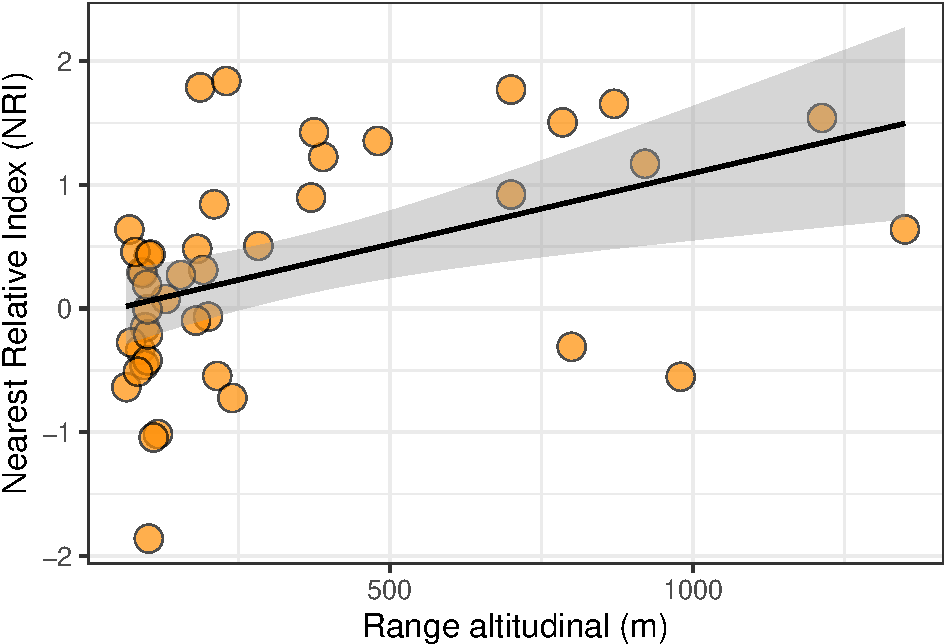
\includegraphics{cap_06_files/figure-latex/unnamed-chunk-3-2.pdf}

\begin{Shaded}
\begin{Highlighting}[]

\CommentTok{\# Gráfico de caixa com a media e os quartis}
\NormalTok{pcaixa  }\OtherTok{\textless{}{-}} \FunctionTok{ggplot}\NormalTok{(penguins, }\FunctionTok{aes}\NormalTok{(}\AttributeTok{y =}\NormalTok{ comprimento\_nadadeira, }\AttributeTok{x =}\NormalTok{ especies )) }\SpecialCharTok{+}
  \FunctionTok{geom\_boxplot}\NormalTok{()}
\NormalTok{pcaixa}
\end{Highlighting}
\end{Shaded}

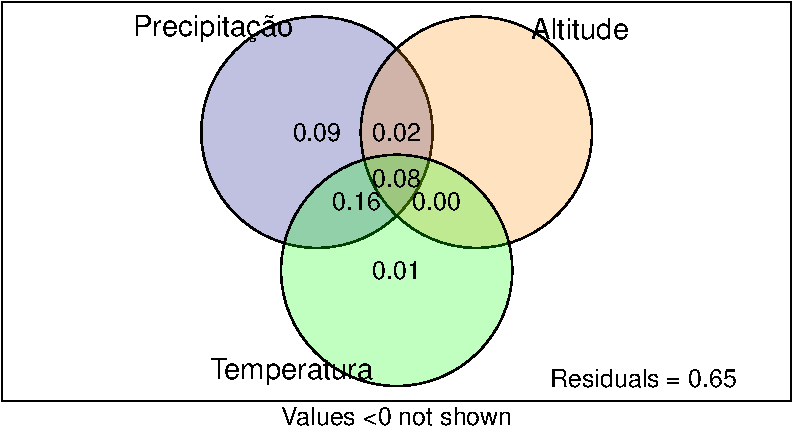
\includegraphics{cap_06_files/figure-latex/unnamed-chunk-3-3.pdf}

\textbf{6.4}
Se você conseguiu resolver o exercício 6.3, agora dê um passo a mais e compare os três gráficos lado a lado utilizando o comando \texttt{grid.arrange}. Lembre-se de colocar um título informativo em cada um dos gráficos antes de juntá-los em uma prancha única. Ao comparar os 3 tipos de gráficos, qual você considera mais informativo? Experimente combinar mais de um ``geom'' e produzir gráficos ainda mais interessantes.

Solução

\begin{Shaded}
\begin{Highlighting}[]
\CommentTok{\# colocando um título em cada gráfico}
\NormalTok{pjitter }\OtherTok{\textless{}{-}}\NormalTok{ pjitter }\SpecialCharTok{+} \FunctionTok{labs}\NormalTok{(}\AttributeTok{title =} \StringTok{"Plot com jitter"}\NormalTok{)}
\NormalTok{pviolin }\OtherTok{\textless{}{-}}\NormalTok{ pviolin }\SpecialCharTok{+} \FunctionTok{labs}\NormalTok{(}\AttributeTok{title =} \StringTok{"Plot com violin"}\NormalTok{)}
\NormalTok{pcaixa  }\OtherTok{\textless{}{-}}\NormalTok{ pcaixa }\SpecialCharTok{+} \FunctionTok{labs}\NormalTok{(}\AttributeTok{title =} \StringTok{"Plot com boxplot"}\NormalTok{)}

\CommentTok{\# juntando os 3 gráficos em um só}
\CommentTok{\# Carregando o pacote gridExtra}
\FunctionTok{library}\NormalTok{(gridExtra)}
\FunctionTok{grid.arrange}\NormalTok{(pjitter, pviolin, pcaixa, }\AttributeTok{ncol =} \DecValTok{3}\NormalTok{)}
\end{Highlighting}
\end{Shaded}

\includegraphics{cap_06_files/figure-latex/unnamed-chunk-4-1.pdf}

Agora misturando as camadas.

\begin{Shaded}
\begin{Highlighting}[]
\CommentTok{\# Misturando geoms}
\FunctionTok{ggplot}\NormalTok{(penguins, }\FunctionTok{aes}\NormalTok{(}\AttributeTok{y =}\NormalTok{ comprimento\_nadadeira, }\AttributeTok{x =}\NormalTok{ especies )) }\SpecialCharTok{+}
  \FunctionTok{geom\_jitter}\NormalTok{(}\AttributeTok{size =}\NormalTok{ .}\DecValTok{5}\NormalTok{, }\AttributeTok{width =}\NormalTok{ .}\DecValTok{2}\NormalTok{, }\FunctionTok{aes}\NormalTok{(}\AttributeTok{color =}\NormalTok{ especies)) }\SpecialCharTok{+}
  \FunctionTok{geom\_boxplot}\NormalTok{(}\FunctionTok{aes}\NormalTok{(}\AttributeTok{fill =}\NormalTok{ especies), }\AttributeTok{alpha =}\NormalTok{ .}\DecValTok{2}\NormalTok{, }\AttributeTok{width =}\NormalTok{ .}\DecValTok{2}\NormalTok{) }\SpecialCharTok{+}
  \FunctionTok{geom\_violin}\NormalTok{(}\AttributeTok{fill =} \StringTok{"gray"}\NormalTok{, }\AttributeTok{alpha =}\NormalTok{ .}\DecValTok{1}\NormalTok{) }\SpecialCharTok{+}
  \FunctionTok{theme\_classic}\NormalTok{(}\AttributeTok{base\_size =} \DecValTok{16}\NormalTok{) }\SpecialCharTok{+}
  \FunctionTok{theme}\NormalTok{(}\AttributeTok{legend.position =} \StringTok{"none"}\NormalTok{) }\SpecialCharTok{+}
  \FunctionTok{labs}\NormalTok{(}\AttributeTok{y =} \StringTok{"Comprimento da nadadeira (mm)"}\NormalTok{,}
       \AttributeTok{x =} \StringTok{"Espécie de pinguim"}\NormalTok{)}
\end{Highlighting}
\end{Shaded}

\includegraphics{cap_06_files/figure-latex/unnamed-chunk-5-1.pdf}

\textbf{6.5}
Utilize o banco de dados \texttt{ecodados::anova\_dois\_fatores} para construir um \href{https://analises-ecologicas.netlify.app/cap6.html\#gr\%C3\%A1fico-de-barras-bar-plot}{gráfico de barras} com a média e o erro padrão do Tempo (Tempo para eliminar a droga do corpo) no eixo Y em funçao da variável Pessoas (XX, ou XY) e Idade (jovem ou idoso). Antes de fazer o gráfico leia com a atenção a descrição do mesmo através do comando \texttt{?ecodados::anova\_dois\_fatores}. Um dica, utilize \texttt{fill} dentro do \texttt{aes} para representar um dos fatores (ex. Pessoas). O outro fator você pode representar no eixo X. Veja se consegue, se não conseguir pode olhar a cola com a solução para aprender como é feito. Outra dica, pesquise sobre a função \texttt{stat\_summary} ela pode te ajudar a calcular a média e o erro padrão dentro do comando que gera o gráfico.

Solução

\begin{Shaded}
\begin{Highlighting}[]
\CommentTok{\# entenda o banco de dados primeiro}
\NormalTok{?ecodados}\SpecialCharTok{::}\NormalTok{anova\_dois\_fatores}
\end{Highlighting}
\end{Shaded}

\textbf{Versão 1}: calculando a média e o erro padrão dentro do próprio gráfico.

\begin{Shaded}
\begin{Highlighting}[]
\FunctionTok{ggplot}\NormalTok{(anova\_dois\_fatores, }\FunctionTok{aes}\NormalTok{(}\AttributeTok{y =}\NormalTok{ Tempo, }\AttributeTok{x =}\NormalTok{ Idade, }\AttributeTok{fill =}\NormalTok{ Pessoas)) }\SpecialCharTok{+}
  \FunctionTok{geom\_point}\NormalTok{(}\AttributeTok{position =} \FunctionTok{position\_dodge}\NormalTok{(}\AttributeTok{width =}\NormalTok{ .}\DecValTok{9}\NormalTok{), }\AttributeTok{size =}\NormalTok{ .}\DecValTok{5}\NormalTok{) }\SpecialCharTok{+}
  \FunctionTok{stat\_summary}\NormalTok{(}\AttributeTok{fun =}\NormalTok{ mean, }\AttributeTok{geom =} \StringTok{"bar"}\NormalTok{, }\AttributeTok{position =} \FunctionTok{position\_dodge}\NormalTok{(}\AttributeTok{width =}\NormalTok{ .}\DecValTok{9}\NormalTok{), }\AttributeTok{alpha =}\NormalTok{ .}\DecValTok{75}\NormalTok{) }\SpecialCharTok{+}
  \FunctionTok{stat\_summary}\NormalTok{(}\AttributeTok{fun.data =}\NormalTok{ mean\_se, }\AttributeTok{geom =} \StringTok{"errorbar"}\NormalTok{, }\AttributeTok{position =} \FunctionTok{position\_dodge}\NormalTok{(}\AttributeTok{width =}\NormalTok{ .}\DecValTok{9}\NormalTok{), }
               \AttributeTok{width =}\NormalTok{ .}\DecValTok{2}\NormalTok{) }\SpecialCharTok{+}
  \FunctionTok{scale\_fill\_manual}\NormalTok{(}\AttributeTok{values =} \FunctionTok{c}\NormalTok{(}\StringTok{"steelblue"}\NormalTok{, }\StringTok{"orange"}\NormalTok{)) }\SpecialCharTok{+}
  \FunctionTok{theme\_bw}\NormalTok{(}\AttributeTok{base\_size =} \DecValTok{16}\NormalTok{) }\SpecialCharTok{+}
  \FunctionTok{labs}\NormalTok{(}\AttributeTok{y =} \StringTok{"Tempo (dias após administração)"}\NormalTok{,}
       \AttributeTok{x =} \StringTok{"Grupo etário"}\NormalTok{)}
\end{Highlighting}
\end{Shaded}

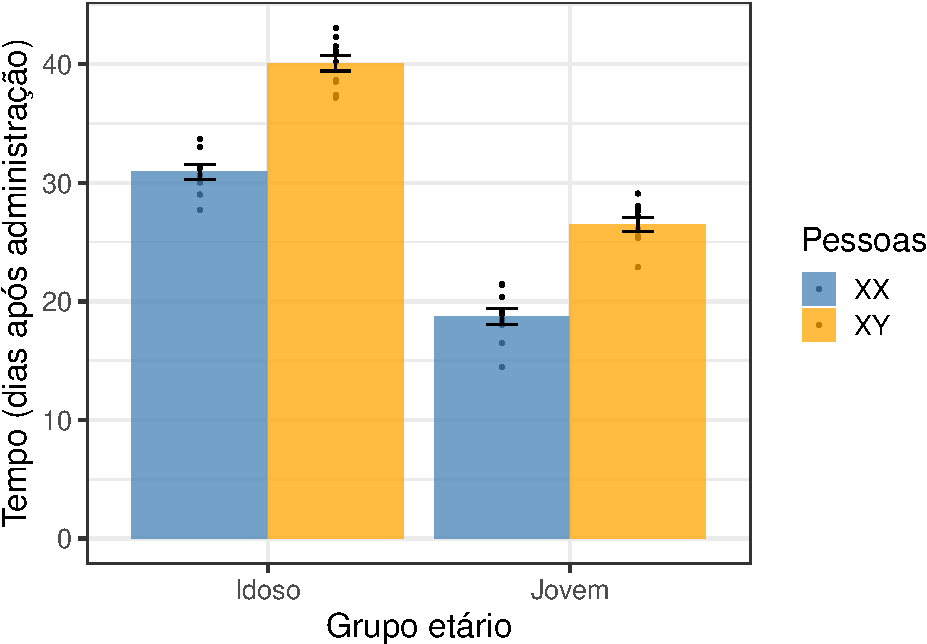
\includegraphics{cap_06_files/figure-latex/unnamed-chunk-7-1.pdf}

\textbf{Versão 2}: calculando a média e o erro padrão antes de produzir o gráfico.

\begin{Shaded}
\begin{Highlighting}[]
\CommentTok{\# Calcular o desvio padrão }
\NormalTok{anova\_media }\OtherTok{\textless{}{-}}\NormalTok{ anova\_dois\_fatores }\SpecialCharTok{\%\textgreater{}\%} 
\NormalTok{    dplyr}\SpecialCharTok{::}\FunctionTok{group\_by}\NormalTok{(Idade, Pessoas ) }\SpecialCharTok{\%\textgreater{}\%} 
\NormalTok{    dplyr}\SpecialCharTok{::}\FunctionTok{summarise}\NormalTok{(}\AttributeTok{media =} \FunctionTok{mean}\NormalTok{(Tempo, }\AttributeTok{na.rm =} \ConstantTok{TRUE}\NormalTok{),}
                     \AttributeTok{desvio =} \FunctionTok{sd}\NormalTok{(Tempo, }\AttributeTok{na.rm =} \ConstantTok{TRUE}\NormalTok{))}
\CommentTok{\#\textgreater{} \textasciigrave{}summarise()\textasciigrave{} has grouped output by \textquotesingle{}Idade\textquotesingle{}. You can override using the \textasciigrave{}.groups\textasciigrave{} argument.}
\CommentTok{\#Veja como ficou }
\FunctionTok{head}\NormalTok{(anova\_media)}
\CommentTok{\#\textgreater{} \# A tibble: 4 x 4}
\CommentTok{\#\textgreater{} \# Groups:   Idade [2]}
\CommentTok{\#\textgreater{}   Idade Pessoas media desvio}
\CommentTok{\#\textgreater{}   \textless{}chr\textgreater{} \textless{}chr\textgreater{}   \textless{}dbl\textgreater{}  \textless{}dbl\textgreater{}}
\CommentTok{\#\textgreater{} 1 Idoso XX       30.9   2.01}
\CommentTok{\#\textgreater{} 2 Idoso XY       40.1   2.04}
\CommentTok{\#\textgreater{} 3 Jovem XX       18.7   2.14}
\CommentTok{\#\textgreater{} 4 Jovem XY       26.5   1.80}
\end{Highlighting}
\end{Shaded}

Agora use esse banco de dados para plotar a média e o erro padrão.

\begin{Shaded}
\begin{Highlighting}[]
\CommentTok{\# Gráfico de barras com desvio padrão}
\FunctionTok{ggplot}\NormalTok{(}\AttributeTok{data =}\NormalTok{ anova\_media, }\FunctionTok{aes}\NormalTok{(}\AttributeTok{y =}\NormalTok{ media, }\AttributeTok{x =}\NormalTok{ Idade, }\AttributeTok{fill =}\NormalTok{ Pessoas)) }\SpecialCharTok{+}
    \FunctionTok{geom\_bar}\NormalTok{(}\AttributeTok{stat =} \StringTok{"identity"}\NormalTok{, }\AttributeTok{alpha =}\NormalTok{ .}\DecValTok{75}\NormalTok{, }\AttributeTok{position =} \FunctionTok{position\_dodge}\NormalTok{()) }\SpecialCharTok{+}
    \FunctionTok{geom\_errorbar}\NormalTok{(}\FunctionTok{aes}\NormalTok{(}\AttributeTok{ymin =}\NormalTok{ media }\SpecialCharTok{{-}}\NormalTok{ desvio, }\AttributeTok{ymax =}\NormalTok{ media }\SpecialCharTok{+}\NormalTok{ desvio), }
                  \AttributeTok{width =}\NormalTok{ .}\DecValTok{1}\NormalTok{, }\AttributeTok{position =} \FunctionTok{position\_dodge}\NormalTok{(}\AttributeTok{width =}\NormalTok{ .}\DecValTok{9}\NormalTok{)) }\SpecialCharTok{+}
  \FunctionTok{scale\_fill\_manual}\NormalTok{(}\AttributeTok{values =} \FunctionTok{c}\NormalTok{(}\StringTok{"steelblue"}\NormalTok{, }\StringTok{"orange"}\NormalTok{)) }\SpecialCharTok{+}
  \FunctionTok{theme\_bw}\NormalTok{(}\AttributeTok{base\_size =} \DecValTok{16}\NormalTok{) }\SpecialCharTok{+}
  \FunctionTok{labs}\NormalTok{(}\AttributeTok{y =} \StringTok{"Tempo (dias após administração)"}\NormalTok{,}
       \AttributeTok{x =} \StringTok{"Grupo etário"}\NormalTok{)}
\end{Highlighting}
\end{Shaded}

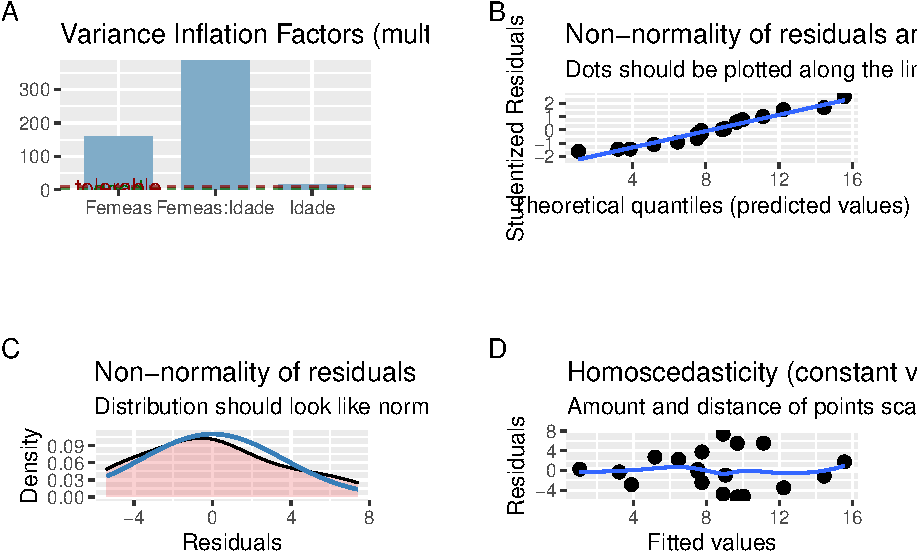
\includegraphics{cap_06_files/figure-latex/unnamed-chunk-9-1.pdf}

\textbf{6.6}
Utilize o banco de dados \texttt{penguins} para criar um \href{https://analises-ecologicas.netlify.app/cap6.html\#gr\%C3\%A1fico-de-dispers\%C3\%A3o-scatter-plot}{gráfico de dispersão} entre o tamanho da nadadeira (eixo Y) e a massa corporal (eixo X). Utilize o argumento \texttt{fill} para ilustrar com cores as diferenças entre os sexos e utilize o comanto \texttt{facte\_grid()} para criar um gráfico separado para cada espécie de pinguim. Se você não conhece essa função, dê uma olhada no help \texttt{?facet\_grid}. Você também pode utilizar a função \texttt{drop\_na()} para excluir os dados faltantes da coluna \texttt{sexo}.

\begin{Shaded}
\begin{Highlighting}[]
\CommentTok{\# primeiro vamos traduizir a coluna sexo para o português}
\NormalTok{penguins}\SpecialCharTok{$}\NormalTok{sexo }\OtherTok{\textless{}{-}} \FunctionTok{fct\_recode}\NormalTok{(penguins}\SpecialCharTok{$}\NormalTok{sexo, }\AttributeTok{masculino =} \StringTok{"male"}\NormalTok{, }\AttributeTok{feminino =} \StringTok{"female"}\NormalTok{)}

\FunctionTok{ggplot}\NormalTok{(penguins }\SpecialCharTok{\%\textgreater{}\%} \FunctionTok{drop\_na}\NormalTok{(sexo), }\FunctionTok{aes}\NormalTok{(}\AttributeTok{y =}\NormalTok{ comprimento\_nadadeira, }\AttributeTok{x =}\NormalTok{ massa\_corporal, }
                                       \AttributeTok{color =}\NormalTok{ sexo, }\AttributeTok{fill =}\NormalTok{ sexo)) }\SpecialCharTok{+}
  \FunctionTok{geom\_point}\NormalTok{(}\AttributeTok{size =}\NormalTok{ .}\DecValTok{4}\NormalTok{) }\SpecialCharTok{+}
  \FunctionTok{geom\_smooth}\NormalTok{(}\AttributeTok{method =}\NormalTok{ lm) }\SpecialCharTok{+}
  \FunctionTok{facet\_grid}\NormalTok{(}\SpecialCharTok{\textasciitilde{}}\NormalTok{especies) }\SpecialCharTok{+}
  \FunctionTok{scale\_color\_manual}\NormalTok{(}\AttributeTok{values =} \FunctionTok{c}\NormalTok{(}\StringTok{"steelblue"}\NormalTok{, }\StringTok{"orange"}\NormalTok{), }\AttributeTok{aesthetics =} \FunctionTok{c}\NormalTok{(}\StringTok{"fill"}\NormalTok{, }\StringTok{"color"}\NormalTok{)) }\SpecialCharTok{+}
  \FunctionTok{theme\_classic}\NormalTok{() }\SpecialCharTok{+}
  \FunctionTok{labs}\NormalTok{(}
    \AttributeTok{y =} \StringTok{"Comprimento da nadadeira (mm)"}\NormalTok{,}
    \AttributeTok{x =} \StringTok{"Massa corporal (g)"}
\NormalTok{  ) }
\end{Highlighting}
\end{Shaded}

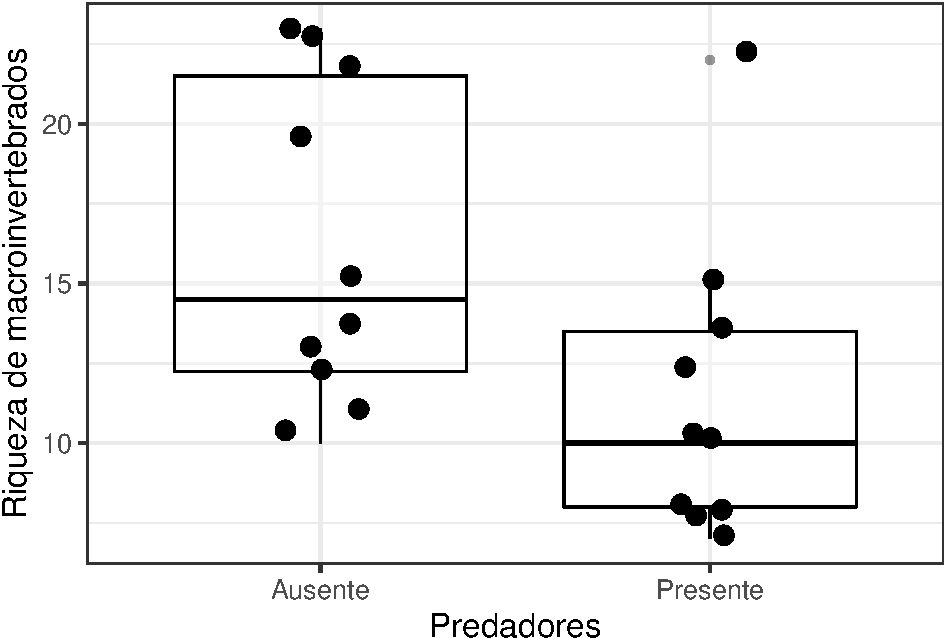
\includegraphics{cap_06_files/figure-latex/unnamed-chunk-10-1.pdf}

\hypertarget{cap.-15---dados-geoespaciais-no-r}{%
\chapter*{Cap. 15 - Dados geoespaciais no R}\label{cap.-15---dados-geoespaciais-no-r}}
\addcontentsline{toc}{chapter}{Cap. 15 - Dados geoespaciais no R}

\textbf{15.1}
Importe o limite dos estados brasileiros no formato \textbf{sf} com o nome \textbf{br}. Para isso, use a função \textbf{ne\_states} do pacote \textbf{rnaturalearth}. Crie um mapa simples cinza utilizando a função \textbf{plot()}, selecionando a coluna \textbf{geometry} com o operador \textbf{\$} e com os argumentos \textbf{axes} e \textbf{graticule} verdadeiros.

Solução:

\begin{Shaded}
\begin{Highlighting}[]
\FunctionTok{library}\NormalTok{(rnaturalearth)}
\NormalTok{br }\OtherTok{\textless{}{-}}\NormalTok{ rnaturalearth}\SpecialCharTok{::}\FunctionTok{ne\_states}\NormalTok{(}\AttributeTok{country =} \StringTok{"Brazil"}\NormalTok{, }\AttributeTok{returnclass =} \StringTok{"sf"}\NormalTok{)}
\FunctionTok{plot}\NormalTok{(br}\SpecialCharTok{$}\NormalTok{geometry, }\AttributeTok{col =} \StringTok{"gray"}\NormalTok{, }\AttributeTok{axes =} \ConstantTok{TRUE}\NormalTok{, }\AttributeTok{graticule =} \ConstantTok{TRUE}\NormalTok{)}
\end{Highlighting}
\end{Shaded}

\includegraphics{cap_15_files/figure-latex/unnamed-chunk-1-1.pdf}

\textbf{15.2}
Dados vetoriais podem ser criados com diversos erros de topologia, e.g., sobreposição de linhas ou polígonos ou buracos. Algumas funções exigem que os objetos vetoriais aos quais são atribuídos esses dados não possuam esses erros para que o algoritmo funcione. Para verificar se há erros, podemos usar a função \textbf{st\_is\_valid()} do pacote \textbf{sf}. Há diversas forma de correções desses erros, mas vamos usar uma correção simples do R, com a função \textbf{st\_make\_valid()}. Vamos fazer essa correção para o \textbf{br} importado anteriormente e atribuindo ao objeto \textbf{br\_valid}. Podemos conferir para saber se há erros e fazer um plot.

Solução:

\begin{Shaded}
\begin{Highlighting}[]
\FunctionTok{library}\NormalTok{(sf)}

\NormalTok{sf}\SpecialCharTok{::}\FunctionTok{st\_is\_valid}\NormalTok{(br)}
\CommentTok{\#\textgreater{}  [1]  TRUE  TRUE  TRUE  TRUE  TRUE  TRUE  TRUE  TRUE  TRUE}
\CommentTok{\#\textgreater{} [10]  TRUE  TRUE  TRUE  TRUE  TRUE  TRUE  TRUE  TRUE  TRUE}
\CommentTok{\#\textgreater{} [19]  TRUE  TRUE  TRUE  TRUE  TRUE FALSE  TRUE  TRUE  TRUE}

\NormalTok{br\_valid }\OtherTok{\textless{}{-}}\NormalTok{ sf}\SpecialCharTok{::}\FunctionTok{st\_make\_valid}\NormalTok{(br)}
\NormalTok{sf}\SpecialCharTok{::}\FunctionTok{st\_is\_valid}\NormalTok{(br\_valid)}
\CommentTok{\#\textgreater{}  [1] TRUE TRUE TRUE TRUE TRUE TRUE TRUE TRUE TRUE TRUE TRUE}
\CommentTok{\#\textgreater{} [12] TRUE TRUE TRUE TRUE TRUE TRUE TRUE TRUE TRUE TRUE TRUE}
\CommentTok{\#\textgreater{} [23] TRUE TRUE TRUE TRUE TRUE}

\FunctionTok{plot}\NormalTok{(br\_valid}\SpecialCharTok{$}\NormalTok{geometry, }\AttributeTok{col =} \StringTok{"gray"}\NormalTok{, }\AttributeTok{axes =} \ConstantTok{TRUE}\NormalTok{, }\AttributeTok{graticule =} \ConstantTok{TRUE}\NormalTok{)}
\end{Highlighting}
\end{Shaded}

\includegraphics{cap_15_files/figure-latex/unnamed-chunk-2-1.pdf}

\textbf{15.3}
Crie um objeto RasterLayer vazio chamado \textbf{ra} com reSolução: de 5º (\textasciitilde600 km). Atribua um sistema de referência de coordendas com o código \textbf{4326}. Atribua valores aleatórios de uma distribuição normal e plote o mesmo.

Solução:

\begin{Shaded}
\begin{Highlighting}[]
\FunctionTok{library}\NormalTok{(raster)}
\NormalTok{ra }\OtherTok{\textless{}{-}}\NormalTok{ raster}\SpecialCharTok{::}\FunctionTok{raster}\NormalTok{(}\AttributeTok{res =} \DecValTok{5}\NormalTok{, }\AttributeTok{crs =} \DecValTok{4326}\NormalTok{)}
\NormalTok{raster}\SpecialCharTok{::}\FunctionTok{values}\NormalTok{(ra) }\OtherTok{\textless{}{-}} \FunctionTok{rnorm}\NormalTok{(raster}\SpecialCharTok{::}\FunctionTok{ncell}\NormalTok{(ra))}
\FunctionTok{plot}\NormalTok{(ra)}
\end{Highlighting}
\end{Shaded}

\includegraphics{cap_15_files/figure-latex/unnamed-chunk-3-1.pdf}

\textbf{15.4}
Reprojete o limite dos estados brasileiros do exercício anterior para o CRS SIRGAS 2000/Brazil Polyconic, utilizando o código EPSG:5880 e chamando de \textbf{br\_poly}. Faça um mapa simples como no exercício 1. Atente para as curvaturas das linhas.

Solução:

\begin{Shaded}
\begin{Highlighting}[]
\FunctionTok{library}\NormalTok{(sf)}
\FunctionTok{library}\NormalTok{(rnaturalearth)}

\NormalTok{br\_valid\_poly }\OtherTok{\textless{}{-}}\NormalTok{ sf}\SpecialCharTok{::}\FunctionTok{st\_transform}\NormalTok{(br\_valid, }\AttributeTok{crs =} \DecValTok{5880}\NormalTok{)}
\FunctionTok{plot}\NormalTok{(br\_valid\_poly}\SpecialCharTok{$}\NormalTok{geometry, }\AttributeTok{col =} \StringTok{"gray"}\NormalTok{, }\AttributeTok{axes =} \ConstantTok{TRUE}\NormalTok{, }\AttributeTok{graticule =} \ConstantTok{TRUE}\NormalTok{)}
\end{Highlighting}
\end{Shaded}

\includegraphics{cap_15_files/figure-latex/unnamed-chunk-4-1.pdf}

\textbf{15.5}
Utilizando a função \textbf{st\_centroid} do pacote \textbf{sf}, crie um vetor chamado \textbf{br\_valid\_cen} que armazenará o centroide de cada estado brasileiro do objeto \textbf{br\_valid} do exercício 2 e plot o resultado.

Solução:

\begin{Shaded}
\begin{Highlighting}[]
\FunctionTok{library}\NormalTok{(sf)}
\FunctionTok{library}\NormalTok{(rnaturalearth)}

\NormalTok{br\_valid\_poly\_cen }\OtherTok{\textless{}{-}}\NormalTok{ sf}\SpecialCharTok{::}\FunctionTok{st\_centroid}\NormalTok{(br\_valid\_poly)}

\FunctionTok{plot}\NormalTok{(br\_valid\_poly}\SpecialCharTok{$}\NormalTok{geometry, }\AttributeTok{col =} \StringTok{"gray"}\NormalTok{, }\AttributeTok{axes =} \ConstantTok{TRUE}\NormalTok{, }\AttributeTok{graticule =} \ConstantTok{TRUE}\NormalTok{)}
\FunctionTok{plot}\NormalTok{(br\_valid\_poly\_cen}\SpecialCharTok{$}\NormalTok{geometry, }\AttributeTok{pch =} \DecValTok{20}\NormalTok{, }\AttributeTok{add =} \ConstantTok{TRUE}\NormalTok{)}
\end{Highlighting}
\end{Shaded}

\includegraphics{cap_15_files/figure-latex/unnamed-chunk-5-1.pdf}

\textbf{15.6}
Ajuste o limite e máscara do objeto raster criado no exercício 3 para o limite do Brasil, atribuindo ao objeto \textbf{ra\_br}. Depois reprojete esse raster para a mesma projeção utilizada no exercício 4 com o nome \textbf{ra\_br\_poly} e plote o mapa resultante.

Solução:

\begin{Shaded}
\begin{Highlighting}[]
\FunctionTok{library}\NormalTok{(raster)}

\NormalTok{ra\_br }\OtherTok{\textless{}{-}}\NormalTok{ ra }\SpecialCharTok{\%\textgreater{}\%} 
\NormalTok{    raster}\SpecialCharTok{::}\FunctionTok{crop}\NormalTok{(br\_valid) }\SpecialCharTok{\%\textgreater{}\%} 
\NormalTok{    raster}\SpecialCharTok{::}\FunctionTok{mask}\NormalTok{(br\_valid)}

\NormalTok{ra\_br\_poly }\OtherTok{\textless{}{-}}\NormalTok{ raster}\SpecialCharTok{::}\FunctionTok{projectRaster}\NormalTok{(ra\_br, }\AttributeTok{crs =} \StringTok{"+init=epsg:5880"}\NormalTok{)}

\FunctionTok{plot}\NormalTok{(ra\_br\_poly)}
\FunctionTok{plot}\NormalTok{(br\_valid\_poly}\SpecialCharTok{$}\NormalTok{geometry, }\AttributeTok{add =} \ConstantTok{TRUE}\NormalTok{)}
\FunctionTok{plot}\NormalTok{(br\_valid\_poly\_cen}\SpecialCharTok{$}\NormalTok{geometry, }\AttributeTok{pch =} \DecValTok{20}\NormalTok{, }\AttributeTok{add =} \ConstantTok{TRUE}\NormalTok{)}
\end{Highlighting}
\end{Shaded}

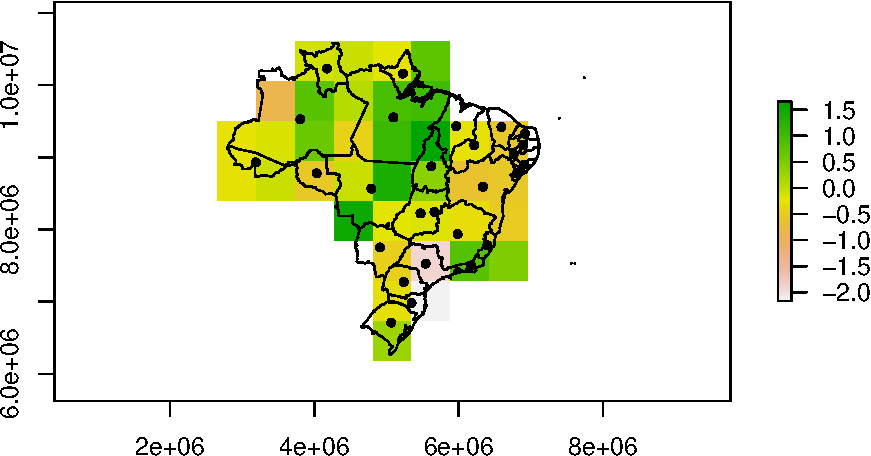
\includegraphics{cap_15_files/figure-latex/unnamed-chunk-6-1.pdf}

\textbf{15.7}
Extraia os valores de cada pixel do raster criado no exercício 6 para os centroides dos estados do Brasil criado no exercício 5, atribuindo à coluna \textbf{val} do objeto espacial chamado \textbf{br\_valid\_poly\_cent\_ra}.

Solução:

\begin{Shaded}
\begin{Highlighting}[]
\NormalTok{br\_valid\_poly\_cent\_ra }\OtherTok{\textless{}{-}}\NormalTok{ br\_valid\_poly\_cen }\SpecialCharTok{\%\textgreater{}\%} 
\NormalTok{    dplyr}\SpecialCharTok{::}\FunctionTok{mutate}\NormalTok{(}\AttributeTok{val =}\NormalTok{ raster}\SpecialCharTok{::}\FunctionTok{extract}\NormalTok{(ra\_br\_poly, .))}
\FunctionTok{head}\NormalTok{(br\_valid\_poly\_cent\_ra}\SpecialCharTok{$}\NormalTok{val)}
\CommentTok{\#\textgreater{} [1]  0.2676713 {-}0.1098317  0.9373188 {-}0.2846465 {-}0.2323340}
\CommentTok{\#\textgreater{} [6] {-}0.4757399}
\end{Highlighting}
\end{Shaded}

\textbf{15.8}
Crie um mapa final usando os resultados dos exercícios 4, 5 e 6. Utilize o pacote \textbf{tmap} e inclua todos os principais elementos de um mapa.

Solução:

\begin{Shaded}
\begin{Highlighting}[]
\FunctionTok{library}\NormalTok{(tmap)}

\FunctionTok{tm\_shape}\NormalTok{(ra\_br\_poly) }\SpecialCharTok{+}
    \FunctionTok{tm\_raster}\NormalTok{(}\AttributeTok{title =} \StringTok{"Raster"}\NormalTok{) }\SpecialCharTok{+}
    \FunctionTok{tm\_shape}\NormalTok{(br\_valid\_poly) }\SpecialCharTok{+}
    \FunctionTok{tm\_borders}\NormalTok{() }\SpecialCharTok{+}
    \FunctionTok{tm\_shape}\NormalTok{(br\_valid\_poly\_cent\_ra) }\SpecialCharTok{+}
    \FunctionTok{tm\_bubbles}\NormalTok{(}\AttributeTok{col =} \StringTok{"val"}\NormalTok{, }\AttributeTok{size =}\NormalTok{ .}\DecValTok{2}\NormalTok{, }\AttributeTok{legend.col.show =} \ConstantTok{FALSE}\NormalTok{) }\SpecialCharTok{+}
    \FunctionTok{tm\_graticules}\NormalTok{(}\AttributeTok{lines =} \ConstantTok{FALSE}\NormalTok{, }
                  \AttributeTok{labels.format =} \FunctionTok{list}\NormalTok{(}\AttributeTok{big.mark =} \StringTok{""}\NormalTok{), }
                  \AttributeTok{labels.rot =} \FunctionTok{c}\NormalTok{(}\DecValTok{0}\NormalTok{, }\DecValTok{90}\NormalTok{),}
                  \AttributeTok{labels.size =}\NormalTok{ .}\DecValTok{7}\NormalTok{) }\SpecialCharTok{+}
    \FunctionTok{tm\_compass}\NormalTok{(}\AttributeTok{position =} \FunctionTok{c}\NormalTok{(}\StringTok{"right"}\NormalTok{, }\StringTok{"top"}\NormalTok{), }\AttributeTok{size =} \DecValTok{2}\NormalTok{) }\SpecialCharTok{+}
    \FunctionTok{tm\_scale\_bar}\NormalTok{(}\AttributeTok{size =} \DecValTok{1}\NormalTok{) }\SpecialCharTok{+}
    \FunctionTok{tm\_xlab}\NormalTok{(}\StringTok{"Longitude"}\NormalTok{, }\AttributeTok{size =} \DecValTok{1}\NormalTok{) }\SpecialCharTok{+}
    \FunctionTok{tm\_ylab}\NormalTok{(}\StringTok{"Latitude"}\NormalTok{, }\AttributeTok{size =} \DecValTok{1}\NormalTok{) }\SpecialCharTok{+}
    \FunctionTok{tm\_credits}\NormalTok{(}\StringTok{"CRS: SIRGAS2000/Policônica"}\NormalTok{, }\AttributeTok{position =} \FunctionTok{c}\NormalTok{(.}\DecValTok{6}\NormalTok{, .}\DecValTok{15}\NormalTok{), }\AttributeTok{size =}\NormalTok{ .}\DecValTok{6}\NormalTok{) }\SpecialCharTok{+}
    \FunctionTok{tm\_credits}\NormalTok{(}\StringTok{"Fonte: Natural Earth (2022)"}\NormalTok{, }\AttributeTok{position =} \FunctionTok{c}\NormalTok{(.}\DecValTok{6}\NormalTok{, .}\DecValTok{12}\NormalTok{), }\AttributeTok{size =}\NormalTok{ .}\DecValTok{6}\NormalTok{) }\SpecialCharTok{+}
    \FunctionTok{tm\_layout}\NormalTok{(}\AttributeTok{main.title =} \StringTok{"Estados do Brasil"}\NormalTok{,}
              \AttributeTok{main.title.position =} \FunctionTok{c}\NormalTok{(.}\DecValTok{1}\NormalTok{, .}\DecValTok{95}\NormalTok{),}
              \AttributeTok{main.title.size =} \FloatTok{1.5}\NormalTok{,}
              \AttributeTok{title.fontface =} \StringTok{"bold"}\NormalTok{,}
              \AttributeTok{legend.position =} \FunctionTok{c}\NormalTok{(}\StringTok{"left"}\NormalTok{, }\StringTok{"bottom"}\NormalTok{),}
              \AttributeTok{legend.title.fontface =} \StringTok{"bold"}\NormalTok{)}
\end{Highlighting}
\end{Shaded}

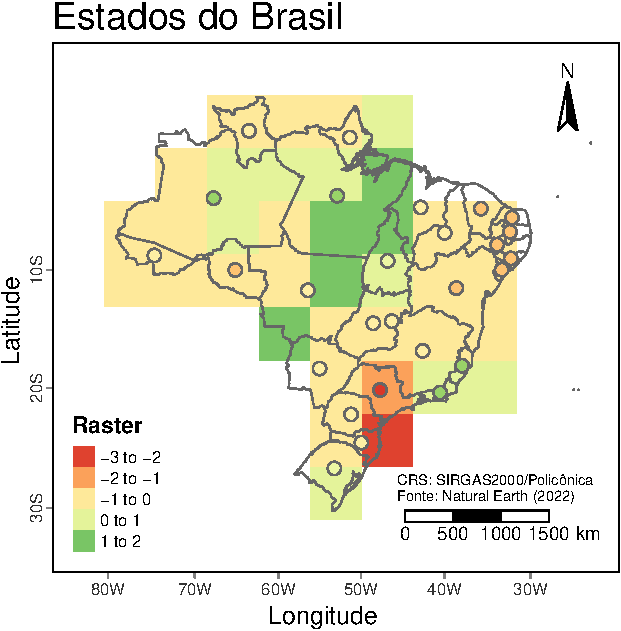
\includegraphics{cap_15_files/figure-latex/unnamed-chunk-8-1.pdf}

  \bibliography{book.bib,packages.bib}

\end{document}
